\documentclass[11pt, a4paper, onecolumn, twoside,french,cleardoublepage=plain,openany]{report}
\usepackage[english]{babel}
\usepackage[a4paper]{geometry}
\usepackage[utf8]{inputenc}
\usepackage[T1]{fontenc}
\usepackage{indentfirst} % alinea on paragraphs
\usepackage[babel=true]{csquotes}
\usepackage{graphicx}
\usepackage[fleqn]{amsmath} % fleqn = align blocs on the left
\usepackage{siunitx} % SI units
\usepackage{amssymb} % for convolution sign
%\usepackage{moreverb} % for c, cpp snippets
\usepackage[pdfusetitle]{hyperref} % for linkable refs and title in pdf meta

%\usepackage[english,boxed,lined,onelanguage]{algorithm2e}
%\SetAlCapSkip{1em} % Margin between algo and caption
%\SetAlCapNameSty{textit} % text style for  algo captions
\usepackage{algpseudocode,algorithm,algorithmicx}

%\usepackage[toc,page]{appendix}
\usepackage{fancyhdr} % For titlepage \lhead, \rhead... 
%\usepackage[font={it}]{caption}
\usepackage[backend=bibtex]{biblatex}
%\bibliography{bibliographie.bib}
%\usepackage{multirow} % Pour colonnes multiples des tableaux
%\usepackage{longtable} % Pour longs tableaux
%\usepackage{array} % Pour \texttt sur tout une colonne
%\usepackage{xcolor} % Pour éviter que footnote ne bug...
%\usepackage{footnote} % Pour les footnotes dans les tableaux
%\makesavenoteenv{tabular} % Pour les footnotes dans les tableaux
%\usepackage{tabularx}
%\usepackage{pdfpages} % Include des pdfs
%\usepackage[nottoc,numbib]{tocbibind} % Pour faire apparaitre la biblio. dans le sommaire

\usepackage{caption}
\usepackage{subcaption}

\usepackage[]{minitoc} % Intermediate 
\usepackage{etoolbox} % For toggle function (to hide titlepage)
\usepackage[acronym,toc,shortcuts]{glossaries}
\usepackage[english]{cleveref} 
%\makeglossary
%\makeindex

\fancypagestyle{titlepage}{% 
	\lhead{
\includegraphics[width=0.30\textwidth]{logos/logo-enseeiht.png}}
	\rhead{
\includegraphics[width=0.30\textwidth]{logos/logo-imt.jpg}}
	\lfoot{
\includegraphics[width=0.28\textwidth]{logos/logo-univ-ups.png}}
	\rfoot{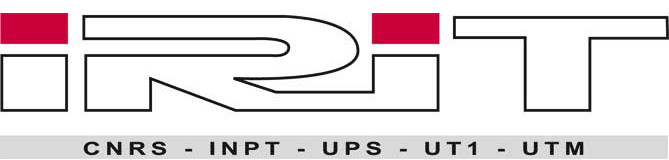
\includegraphics[width=0.28\textwidth]{logos/logo-irit.jpg}}
	\fancyhead[C]{} % On enlève les informations du header
	\fancyfoot[C]{} % On enlève les informations du footer
	\renewcommand{\headrulewidth}{0pt} % On enlève la ligne du header
} \Huge
\fancypagestyle{body}{%
	\restoregeometry 
	\pagestyle{fancy}
	\fancyhf{}
	\fancyhead[LO]{\ifthenelse{\equal{\value{chapter}}{0}}{}{\thesection. \rightmark}} %rightmark = section
	\fancyhead[RE]{\ifthenelse{\equal{\value{chapter}}{0}}
		{}
		{Chapter \thechapter.}
		\leftmark
	} %leftmark = chapter
	\fancyhead[RO]{\thepage} %
	\fancyhead[LE]{\thepage} %
	\renewcommand*{\chaptermark}[1]{\markboth{##1}{}}
	\renewcommand*{\sectionmark}[1]{\markright{##1}{}}
	\renewcommand\headrulewidth{.1pt}
%	\setlength{\parskip}{0.3cm} % Espace entre paragraphes
%	\renewcommand{\arraystretch}{1.5} % Espace entre cases d'un tableau
}
\fancypagestyle{plain}{
	\pagestyle{body}
	\fancyhead[LO]{\rightmark}
}
\fancypagestyle{appendix}{%
	\restoregeometry
	% On nettoie les headers et footers existants de "fancy"
	\fancyhf{}
	% Pour le header
	\fancyhead[RE]{Appendix}
	\fancyhead[LO]{\thechapter. \leftmark} %leftmark = chapter
	\fancyhead[RO]{\thepage} %
	\fancyhead[LE]{\thepage} %
	\renewcommand*{\chaptermark}[1]{\markboth{##1}{}}
	\renewcommand\headrulewidth{.1pt}
	% Pour le footer
	%\fancyfoot[C]{\thepage}
	\renewcommand\footrulewidth{0pt}
}
% \newacronymwithdescr{Label}{Court}{Long}{Description}
\newcommand*{\newacronymwithdescr}[5][]{%
  \newglossaryentry{main-#2}{name={#3},%
  text={(\acs{#2}) #3\glsadd{#2}},%
  description={#5},%
  #1
  }%
  \newacronym{#2}{#3\glsadd{main-#2}}{#4}%
}

% Pas de point final pour les entrées glossaire ou acronymes
\setacronymstyle{sm-short-long}
%\newacronym{IMT}{IMT}{Institut de Mathématiques de Toulouse}
\newacronymwithdescr{IMT}{IMT}{Institut de Mathématiques de Toulouse}{is the main laboratory in mathematics in Toulouse}
\newglossaryentry{Blabla}{name=Blabla,description={is....}}

% To use the glossary entries:
% \acs{} (for short one)
% \ac{} (for long one - only on first appearence)


% MACROS

% Couleurs pour les corrections
\newcommand {\JY}[1] {\textcolor{red}{#1}}
\newcommand {\FR}[1] {\textcolor[rgb]{0.0,0.3,0.0}{#1}}
\newcommand {\OL}[1] {\textcolor{blue}{#1}}
\newcommand {\HW}[1] {\textcolor[rgb]{0.3,0.2,0.0}{#1}}
%\newcommand{\hilite}[1] {\emph{#1}}
\newcommand{\hilite}[1] {\Req{#1}}
\newcommand {\Req}[1] {\textcolor[rgb]{0.75,0.0,0.0}{#1}}
\newcommand {\Geq}[1] {\textcolor[rgb]{0.0,0.5,0.0}{#1}}
\newcommand {\Beq}[1] {\textcolor[rgb]{0.0,0.15,0.60}{#1}}
\newcommand {\black}[1] {\textcolor{black}{#1}}

% Espaces mathématiques
\newcommand {\DPUN} {{\mathcal D}}
\newcommand {\DTREE} {{\mathcal D}^e}
\newcommand {\CC} {\mathbb C}
\newcommand {\RR} {\mathbb R}
\newcommand {\RP} {\mathbb R^{\mathcal P}}
\newcommand {\RPE} {\mathbb R^{\mathcal P \times |\edges |}}
\newcommand {\codeset} {\mathbb R^{\mathcal P \times \leaves}}
\newcommand {\Dset} {\mathbb R^{\mathcal P \times (\mathcal P \#\leaves) }}
\newcommand {\ZZ} {\mathbb Z}
\newcommand {\NN} {\mathbb N}
\newcommand {\PP} {{\mathcal P}}
\newcommand {\HH} {{\mathbb H}}
\newcommand {\II} {{\mathbb I}}
\renewcommand {\SS} {{\mathcal S}} % applis supports
\newcommand {\SA} {{\mathbb S}} % support accessible

% Fonctions
\newcommand {\f}[1] { {\mathcal F}\left( #1 \right) }
\newcommand {\F}[1] { {\mathcal F^{-1}}\left( #1 \right) }
\newcommand {\norm}[2] {\left\| #1 \right\| _{#2}}
\newcommand {\defeq} {\triangleq}

% Opérateurs
\DeclareMathOperator {\sign} {sign}
\DeclareMathOperator {\prox} {prox}
\DeclareMathOperator {\argmin} {argmin}
\DeclareMathOperator {\supp} {supp}
\DeclareMathOperator {\rg} {rg}
\DeclareMathOperator {\diag} {diag}
\newcommand {\RG}[1] {\rg\left( #1 \right)}
\newcommand {\SUPP}[1] {\supp\left( #1 \right)}
\newcommand {\PS}[2] {\langle #1 , #2 \rangle}
\newcommand {\PROBA}[1] {\mathbb P \left( #1 \right)}
\newcommand {\one}[1] {\mathbbm{1}_{ #1 }}
%\newcommand {\one}[1] {\chi_{ #1 }} %{\mathbbm{1}_{ #1 }}
\newcommand {\oneinf}[1] {\chi_{ #1 }}
%\newcommand {\oneinf}[1] {{\mathcal I}_{ #1 }} 

% Acronymes
\newcommand {\PSNR} { \textrm{PSNR}^* } 
\newcommand {\NRE} { \textrm{NRE} }
\newcommand {\CPR} { \textrm{RER} }
\newcommand {\COST} { \textrm{G} } % ancien compression ratio

% Raccourcis
\newtheorem{prop}{Proposition}[section]

\newcommand {\nodes} {\mathcal N}
\newcommand {\edges} {\mathcal E}
\newcommand {\leaves} {\mathcal L}
\newcommand {\NL} {\#\leaves}
\newcommand {\hall} {h^e _{e \in \edges}}
%\newcommand {\multiconv}[1] { \bigstar_{\substack{#1}}\, }
\newcommand {\multiconv}[1] { \mathbf h^{#1}\, }
\newcommand {\tpath}[1] {\mathcal{C}(#1)}
\newcommand {\code} {\mathbf x}
\newcommand {\data} {\mathbf y}
\newcommand {\dataex} {\mathbf b}
\newcommand {\databis} {\mathbf y^e}
\newcommand {\D} {\mathbf D}
\newcommand {\Hs} {\mathbf A}
\newcommand {\Ha} {\mathbf H}
\newcommand {\Haf} {\hat{\mathbf H}}
\newcommand {\Hab} {\bar{\mathbf H}}
\newcommand {\res} {\mathbf r}

\newcommand {\tree}{\mathcal T}
\newcommand{\subtree}[1]{\tree^{#1}}

\newcommand {\stopalgo}{\epsilon}

% autres MACROS
\newcommand {\hkall} {(h^k)_{1 \leq k \leq K}}
\newcommand {\hkconv} {h^1 * \dots * h^K}
\newcommand {\hkconvnorm} {\frac{h^1}{\norm{h^1}{2}} * \dots * \frac{h^K}{\norm{h^K}{2}}}
\newcommand {\hkconvp} {g^{1} * \dots * g{K}}
\newcommand {\hkconvs} {f^{1} * \dots * f^{K}}
\newcommand {\fobj} {\| \code * h^1 * \dots * h^K - \data \|_2^2}
\newcommand {\fobjlambda} {\| \lambda \code * h^1 * \dots * h^K - \data \|_2^2}

% Macros added by Mael
\newcommand{\file}{\texttt}
\newcommand{\dispCode}{\texttt}
\newcommand{\dispCodeLong}[1]{
\begin{verbatim} #1 \end{verbatim}
}
\DeclareMathOperator*{\argmax}{\arg\!\max}% http://tex.stackexchange.com/q/83169/5764

\algnewcommand\algorithmicinput{\textbf{Input:}}
\algnewcommand\Input{\item[\algorithmicinput]}
\algnewcommand\algorithmicoutput{\textbf{Output:}}
\algnewcommand\Output{\item[\algorithmicoutput]}

 % <-- all the \usepackages
\fancypagestyle{titlepage}{% 
	\lhead{
\includegraphics[width=0.30\textwidth]{logos/logo-enseeiht.png}}
	\rhead{
\includegraphics[width=0.30\textwidth]{logos/logo-imt.jpg}}
	\lfoot{
\includegraphics[width=0.28\textwidth]{logos/logo-univ-ups.png}}
	\rfoot{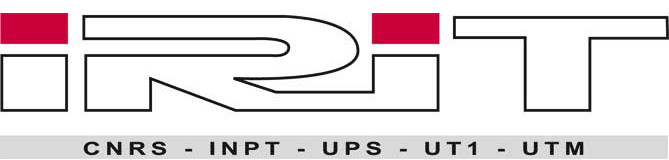
\includegraphics[width=0.28\textwidth]{logos/logo-irit.jpg}}
	\fancyhead[C]{} % On enlève les informations du header
	\fancyfoot[C]{} % On enlève les informations du footer
	\renewcommand{\headrulewidth}{0pt} % On enlève la ligne du header
} \Huge
\fancypagestyle{body}{%
	\restoregeometry 
	\pagestyle{fancy}
	\fancyhf{}
	\fancyhead[LO]{\ifthenelse{\equal{\value{chapter}}{0}}{}{\thesection. \rightmark}} %rightmark = section
	\fancyhead[RE]{\ifthenelse{\equal{\value{chapter}}{0}}
		{}
		{Chapter \thechapter.}
		\leftmark
	} %leftmark = chapter
	\fancyhead[RO]{\thepage} %
	\fancyhead[LE]{\thepage} %
	\renewcommand*{\chaptermark}[1]{\markboth{##1}{}}
	\renewcommand*{\sectionmark}[1]{\markright{##1}{}}
	\renewcommand\headrulewidth{.1pt}
%	\setlength{\parskip}{0.3cm} % Espace entre paragraphes
%	\renewcommand{\arraystretch}{1.5} % Espace entre cases d'un tableau
}
\fancypagestyle{plain}{
	\pagestyle{body}
	\fancyhead[LO]{\rightmark}
}
\fancypagestyle{appendix}{%
	\restoregeometry
	% On nettoie les headers et footers existants de "fancy"
	\fancyhf{}
	% Pour le header
	\fancyhead[RE]{Appendix}
	\fancyhead[LO]{\thechapter. \leftmark} %leftmark = chapter
	\fancyhead[RO]{\thepage} %
	\fancyhead[LE]{\thepage} %
	\renewcommand*{\chaptermark}[1]{\markboth{##1}{}}
	\renewcommand\headrulewidth{.1pt}
	% Pour le footer
	%\fancyfoot[C]{\thepage}
	\renewcommand\footrulewidth{0pt}
}
% \newacronymwithdescr{Label}{Court}{Long}{Description}
\newcommand*{\newacronymwithdescr}[5][]{%
  \newglossaryentry{main-#2}{name={#3},%
  text={(\acs{#2}) #3\glsadd{#2}},%
  description={#5},%
  #1
  }%
  \newacronym{#2}{#3\glsadd{main-#2}}{#4}%
}

% Pas de point final pour les entrées glossaire ou acronymes
\setacronymstyle{sm-short-long}
%\newacronym{IMT}{IMT}{Institut de Mathématiques de Toulouse}
\newacronymwithdescr{IMT}{IMT}{Institut de Mathématiques de Toulouse}{is the main laboratory in mathematics in Toulouse}
\newglossaryentry{Blabla}{name=Blabla,description={is....}}

% To use the glossary entries:
% \acs{} (for short one)
% \ac{} (for long one - only on first appearence)


% MACROS

% Couleurs pour les corrections
\newcommand {\JY}[1] {\textcolor{red}{#1}}
\newcommand {\FR}[1] {\textcolor[rgb]{0.0,0.3,0.0}{#1}}
\newcommand {\OL}[1] {\textcolor{blue}{#1}}
\newcommand {\HW}[1] {\textcolor[rgb]{0.3,0.2,0.0}{#1}}
%\newcommand{\hilite}[1] {\emph{#1}}
\newcommand{\hilite}[1] {\Req{#1}}
\newcommand {\Req}[1] {\textcolor[rgb]{0.75,0.0,0.0}{#1}}
\newcommand {\Geq}[1] {\textcolor[rgb]{0.0,0.5,0.0}{#1}}
\newcommand {\Beq}[1] {\textcolor[rgb]{0.0,0.15,0.60}{#1}}
\newcommand {\black}[1] {\textcolor{black}{#1}}

% Espaces mathématiques
\newcommand {\DPUN} {{\mathcal D}}
\newcommand {\DTREE} {{\mathcal D}^e}
\newcommand {\CC} {\mathbb C}
\newcommand {\RR} {\mathbb R}
\newcommand {\RP} {\mathbb R^{\mathcal P}}
\newcommand {\RPE} {\mathbb R^{\mathcal P \times |\edges |}}
\newcommand {\codeset} {\mathbb R^{\mathcal P \times \leaves}}
\newcommand {\Dset} {\mathbb R^{\mathcal P \times (\mathcal P \#\leaves) }}
\newcommand {\ZZ} {\mathbb Z}
\newcommand {\NN} {\mathbb N}
\newcommand {\PP} {{\mathcal P}}
\newcommand {\HH} {{\mathbb H}}
\newcommand {\II} {{\mathbb I}}
\renewcommand {\SS} {{\mathcal S}} % applis supports
\newcommand {\SA} {{\mathbb S}} % support accessible

% Fonctions
\newcommand {\f}[1] { {\mathcal F}\left( #1 \right) }
\newcommand {\F}[1] { {\mathcal F^{-1}}\left( #1 \right) }
\newcommand {\norm}[2] {\left\| #1 \right\| _{#2}}
\newcommand {\defeq} {\triangleq}

% Opérateurs
\DeclareMathOperator {\sign} {sign}
\DeclareMathOperator {\prox} {prox}
\DeclareMathOperator {\argmin} {argmin}
\DeclareMathOperator {\supp} {supp}
\DeclareMathOperator {\rg} {rg}
\DeclareMathOperator {\diag} {diag}
\newcommand {\RG}[1] {\rg\left( #1 \right)}
\newcommand {\SUPP}[1] {\supp\left( #1 \right)}
\newcommand {\PS}[2] {\langle #1 , #2 \rangle}
\newcommand {\PROBA}[1] {\mathbb P \left( #1 \right)}
\newcommand {\one}[1] {\mathbbm{1}_{ #1 }}
%\newcommand {\one}[1] {\chi_{ #1 }} %{\mathbbm{1}_{ #1 }}
\newcommand {\oneinf}[1] {\chi_{ #1 }}
%\newcommand {\oneinf}[1] {{\mathcal I}_{ #1 }} 

% Acronymes
\newcommand {\PSNR} { \textrm{PSNR}^* } 
\newcommand {\NRE} { \textrm{NRE} }
\newcommand {\CPR} { \textrm{RER} }
\newcommand {\COST} { \textrm{G} } % ancien compression ratio

% Raccourcis
\newtheorem{prop}{Proposition}[section]

\newcommand {\nodes} {\mathcal N}
\newcommand {\edges} {\mathcal E}
\newcommand {\leaves} {\mathcal L}
\newcommand {\NL} {\#\leaves}
\newcommand {\hall} {h^e _{e \in \edges}}
%\newcommand {\multiconv}[1] { \bigstar_{\substack{#1}}\, }
\newcommand {\multiconv}[1] { \mathbf h^{#1}\, }
\newcommand {\tpath}[1] {\mathcal{C}(#1)}
\newcommand {\code} {\mathbf x}
\newcommand {\data} {\mathbf y}
\newcommand {\dataex} {\mathbf b}
\newcommand {\databis} {\mathbf y^e}
\newcommand {\D} {\mathbf D}
\newcommand {\Hs} {\mathbf A}
\newcommand {\Ha} {\mathbf H}
\newcommand {\Haf} {\hat{\mathbf H}}
\newcommand {\Hab} {\bar{\mathbf H}}
\newcommand {\res} {\mathbf r}

\newcommand {\tree}{\mathcal T}
\newcommand{\subtree}[1]{\tree^{#1}}

\newcommand {\stopalgo}{\epsilon}

% autres MACROS
\newcommand {\hkall} {(h^k)_{1 \leq k \leq K}}
\newcommand {\hkconv} {h^1 * \dots * h^K}
\newcommand {\hkconvnorm} {\frac{h^1}{\norm{h^1}{2}} * \dots * \frac{h^K}{\norm{h^K}{2}}}
\newcommand {\hkconvp} {g^{1} * \dots * g{K}}
\newcommand {\hkconvs} {f^{1} * \dots * f^{K}}
\newcommand {\fobj} {\| \code * h^1 * \dots * h^K - \data \|_2^2}
\newcommand {\fobjlambda} {\| \lambda \code * h^1 * \dots * h^K - \data \|_2^2}

% Macros added by Mael
\newcommand{\file}{\texttt}
\newcommand{\dispCode}{\texttt}
\newcommand{\dispCodeLong}[1]{
\begin{verbatim} #1 \end{verbatim}
}
\DeclareMathOperator*{\argmax}{\arg\!\max}% http://tex.stackexchange.com/q/83169/5764

\algnewcommand\algorithmicinput{\textbf{Input:}}
\algnewcommand\Input{\item[\algorithmicinput]}
\algnewcommand\algorithmicoutput{\textbf{Output:}}
\algnewcommand\Output{\item[\algorithmicoutput]}
\author{Maël Valais}
\date{Updated on \today}
\title{Optimization of dictionaries structured in convolutional trees for sparse image representation - Master's Thesis}
\begin{document}
%\begin{titlepage}
\thispagestyle{pagedegarde}
\newgeometry{tmargin=2.2cm,bmargin=4cm,lmargin=2cm,rmargin=2cm}
\begin{center}
\topskip2.8cm
\textsc{Université Toulouse III — Paul Sabatier}\\
\vspace{0.5 cm}
\line(1,0){100}\\
\vspace{0.6 cm}
{{{Internship Report}}}\\
\vspace{0.3cm}
Defended on September 15\th, 2016\\ \vspace{0.3 cm} par\\ \vspace{0.3 cm} \textbf{Maël \textsc{Valais}}\\
\vfill
{\Huge \textbf{Optimization of dictionaries structured as convolutions trees for sparse image representation }}\\
\vfill

{{Internship at \acs{IMT}}}\\
{Université Paul Sabatier}\\
{118, route de Narbonne}\\
{31400 Toulouse}\\
\vspace{2 cm}

\par Supervised by \\ \textbf{François \textsc{Malgouyres}}\\
Institut de Mathématiques de Toulouse\\ 
%\vspace{1cm}
\par and \\Jean-Yves \textbf{ \textsc{Tourneret}}\\
ENSEIHHT, Toulouse
\end{center}
\end{titlepage}

% Préparation pour les pages de corps
\pagestyle{empty}
\restoregeometry
\cleardoublepage % Blanc jusqu'à prochaîne page paire

\tableofcontents
{\let\clearpage\relax\listoffigures}
{\let\clearpage\relax\listoftables}
{\let\clearpage\relax\listofalgorithms}

\pagestyle{corps} % Uncomment to show title page
\pagestyle{body}
\tableofcontents

\chapter{Introduction}

\section{The need for sparse representations}

A sparse signal over some representation means that it can be written with as few information as possible – in other words, sparse means with many zeros. Many applications spanning from machine learning to image denoising heavily rely on the property that we can summarize – or more precisely approximate, or factorize – any signal using a proper representation. The job of obtaining the raw\footnote{Any raw signal is actually represented by the canonical basis} signal from its sparse counterpart takes the form of an operator, often called dictionary or transform.

The Fourier transform is an ideal example of such operators. In figure \ref{explefourier}, the left picture $y$ has been represented using a Fourier basis, which can be written as a matrix $D$. The right picture shows the coefficients $x$ such that
$$D^Ty = x$$
\begin{figure}[!h]
\subcaptionbox{A picture featuring a blackboard at INSA Toulouse}%
  [.49\linewidth]{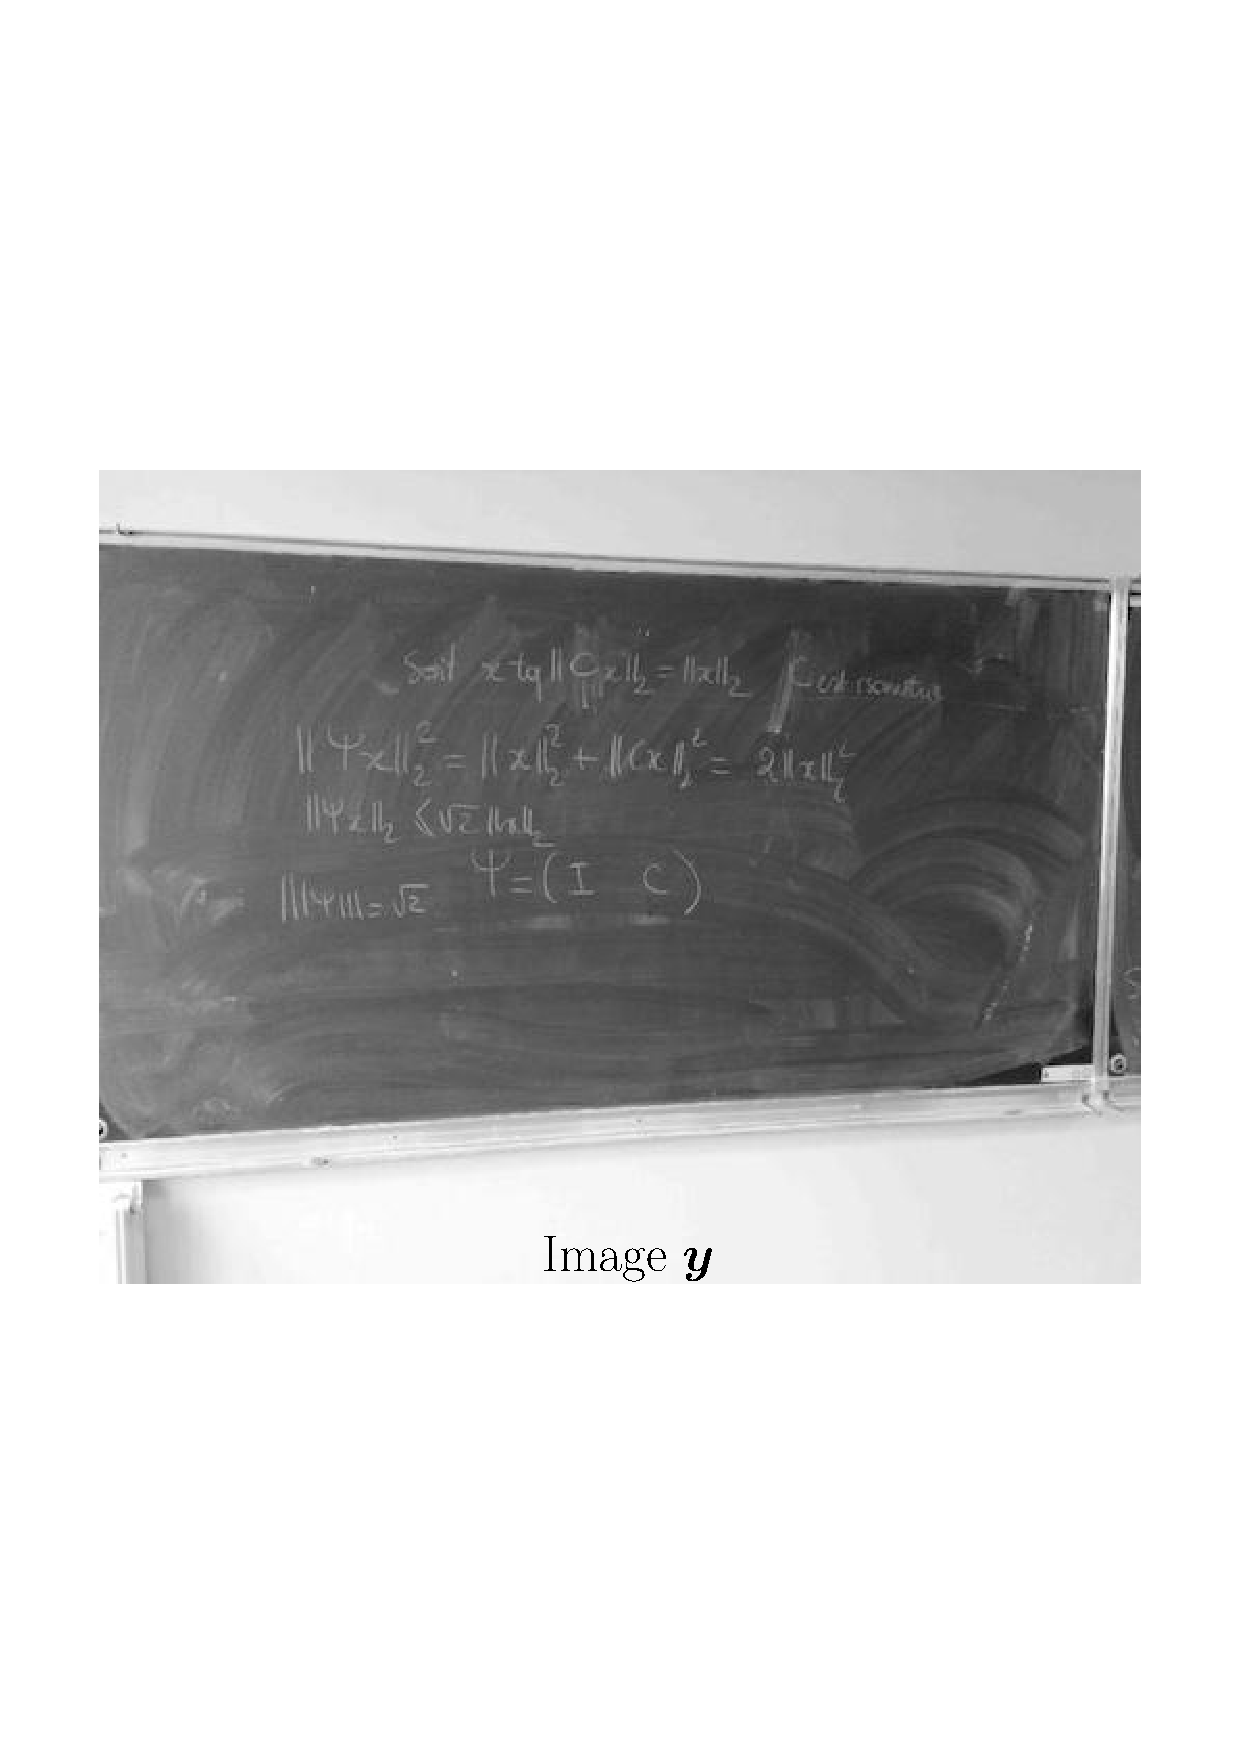
\includegraphics[width=0.49\textwidth]{figures/exple_fourier_spacial.pdf}}
 \subcaptionbox{Frequential representation of the blackboard using Fourier transform. Middle coefficients are coding for general and constant features of the picture while the corner values are coding for the details. The multiple white lines, spanning from the middle to the borders, outline the discontinuities caused by the edges of the blackboard.}%
  [.49\linewidth]{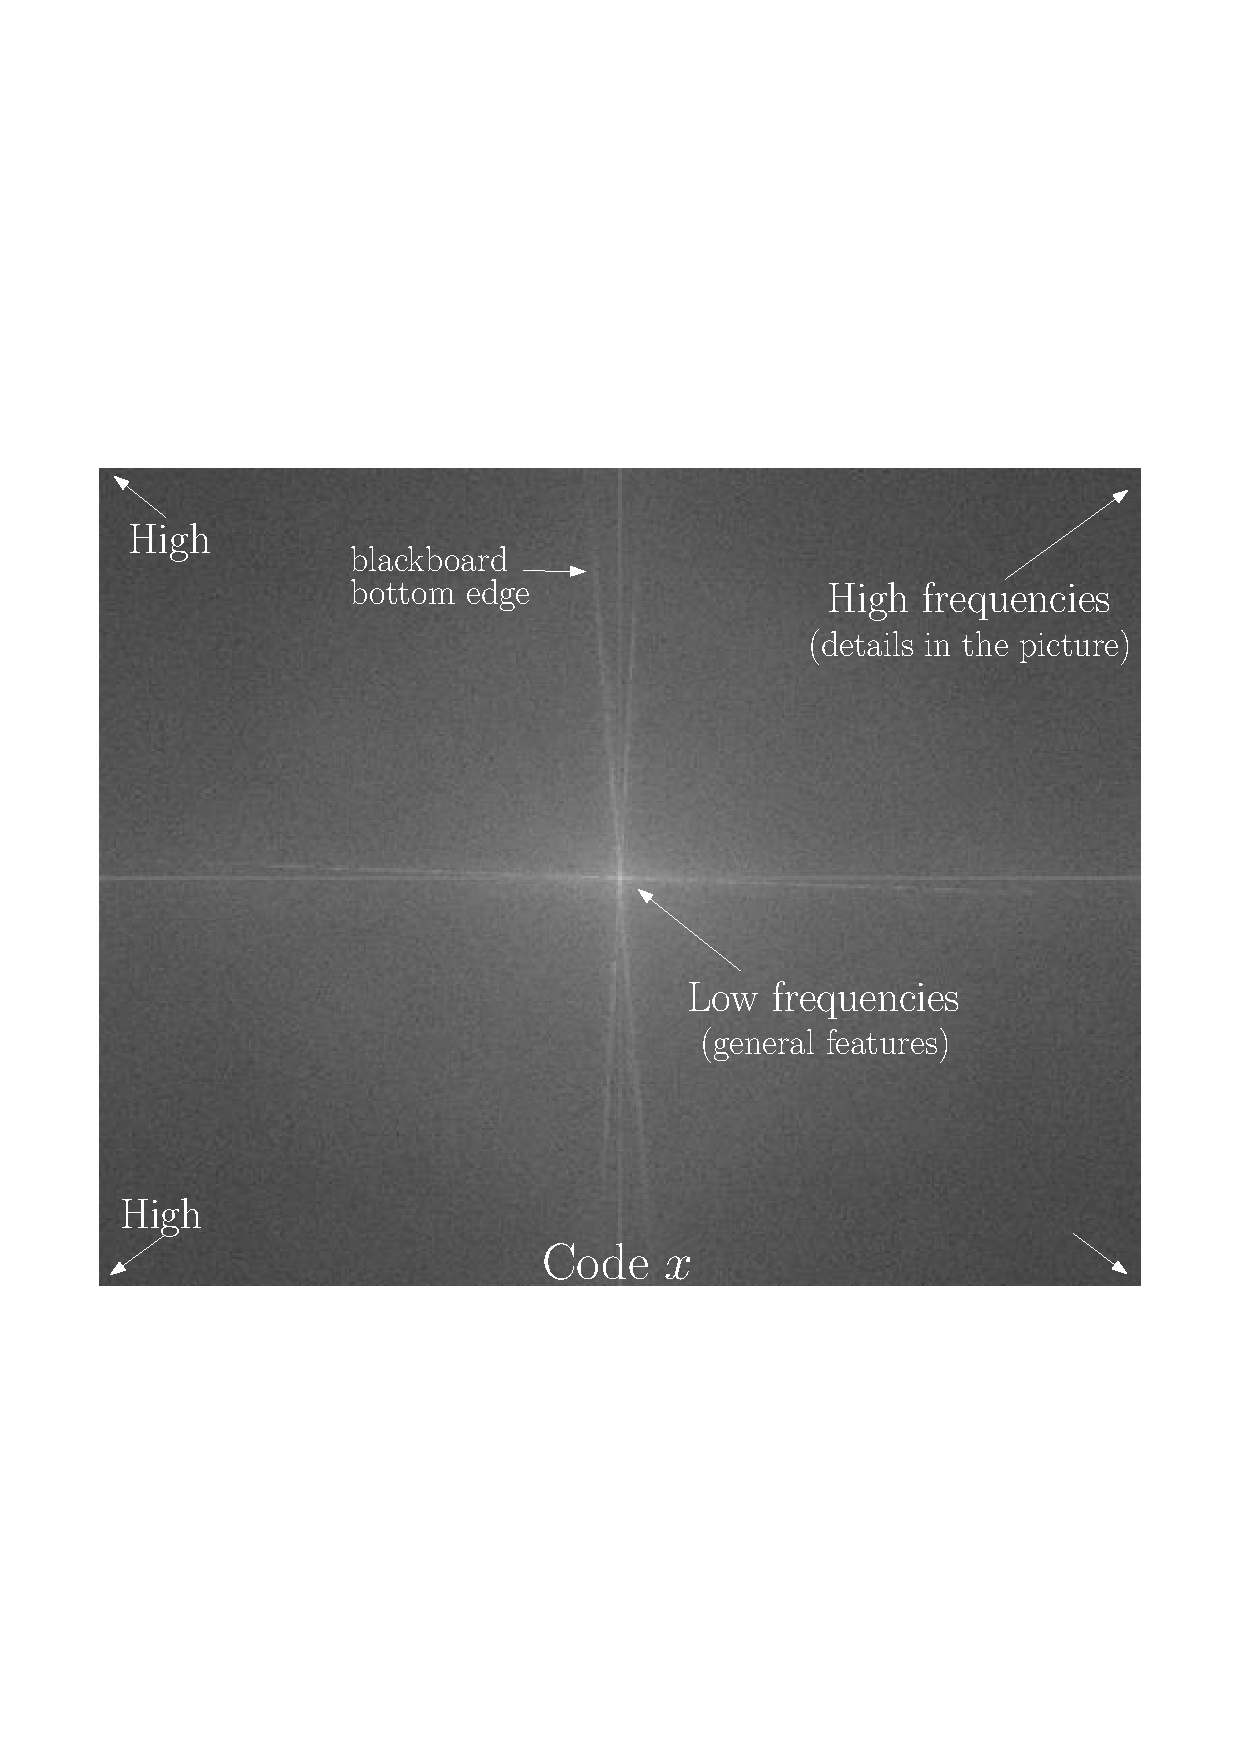
\includegraphics[width=0.49\textwidth]{figures/exple_fourier_frequen.pdf}}
  \caption{ ($D^Ty=x$) Example of decomposition of a signal $y$ using the dictionary $D$ made of Fourier series.} \label{explefourier}
\end{figure}
But the Fourier transform is quite different from our convolutional tree structure. First, it's a linear mapping and its associated matrix forms a basis. This implies bijectivity: every code $x$ has a unique image $y$. Also, Fourier's basis is orthogonal, meaning that the operator is stable (it does amplify errors). Finally, the basis is normed, meaning that ...

More importantly, Fourier has interesting properties that allow fast implementations. For example, using \texttt{fft2} on matlab is extremely fast. Instead of computing an time-expensive $O(N^2)$\footnote{$N$ is the dimension of the "flatten" image, if we consider the image as a vector} matrix-vector product, the fast Fourier transform only require a $O(NlogN)$ time.

The Fourier transform is widely used as an operator for sparse representations, mainly in fields dealing with regular signals that can be approximated by a sum of sines. But this operator does not do well on images: they contain many discontinuities and are far from being representable using sines. In \ref{fig_} Also, we can see that the right picture doesn't seem to be sparse: many coefficients are non-zeros.

Many other non-adaptative dictionaries exist, like the cosine transform (used by JPEG), the wavelet transform (used by JPEG2000, heavily used for encoding movies in theaters) or the curvelet transform. And as for the Fourier transform, these operators are known to be fast.

\section{Adaptative dictionaries}
As mentioned, analytically-based dictionaries do not produce sparse representations for every kind of signal, although allowing low computational time. Dictionary learning tries to address the adaptativeness issue. Instead of using basis matrices, we allow ourselves to use overcomplete dictionaries (more columns than lines) made of learned images (the atoms).
\begin{figure}[!h] \centering
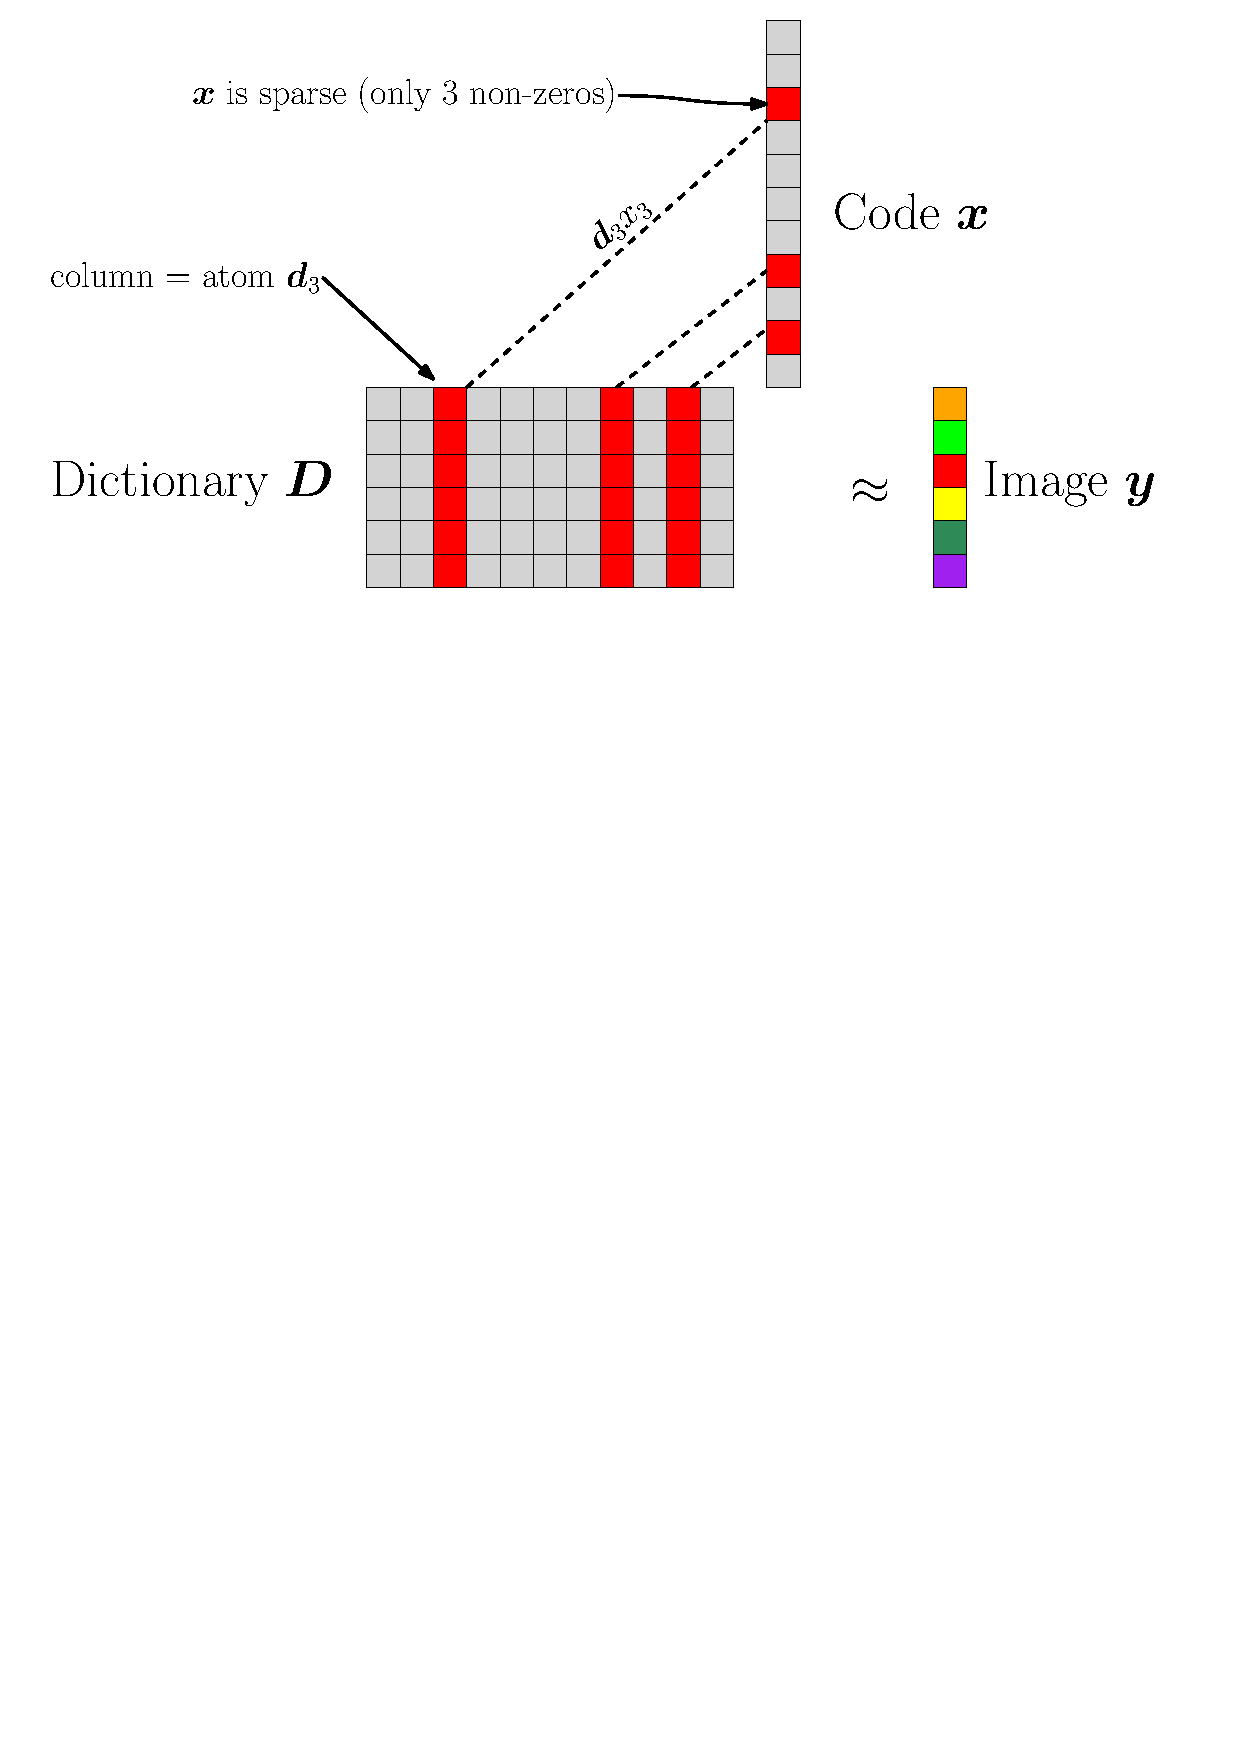
\includegraphics[width=0.5\textwidth]{figures/sparsity-matrix.pdf}
\caption{Matrix view of $Dx$ when $D$ is overcomplete (much more columns/atoms than lines, which is the dimension of the signal $y$) \label{fig_overcomplete_matrix}}
\end{figure}
In figure \ref{fig_overcomplete_matrix}, the sparse code is multiplied to $D$ to give an approximation of $y$. Finding a good dictionary amounts to find the best atoms in $D$ such that every $y$ gives a good sparse representation – or code – $x$.

More formally, the dictionary learning problem is defined by
\begin{equation*}
\begin{aligned}
(DL) && \underset{D,x}{\min} \lambda \lVert x \rVert + \lVert Dx-y \rVert^2
\end{aligned}
\end{equation*}
\ac{KSVD} is a very well known algorithm for dictionary learning. Instead of having a pre-determined $D$, we are going to learn it.

As many of the concepts behind the PALMTREE algorithm developed in \cite{chabiron_optimization_2016} come from the K-SVD algorithm, the next section will introduce it.


\section{\ac{KSVD} algorithm}

K-SVD learns the dictionary by alternatively optimizing $x$ and $D$. Optimizing $x$ is the sparse coding phase, and optimizing $D$ is the dictionary update phase.


\begin{algorithm} % XXX Finish algorithm
    \caption{K-SVD (K-Singular Value Decomposition) algorithm for dictionary learning}
  \begin{algorithmic}[1]
    \Input learning signals $(y_i)_{i=1..N}$ forming columns of $Y \in \mathbb{R}^{n \times N}$
    \Output dictionary $D \in \mathbb{R}^{n \times K}$ with $K>>n$
    \State \textbf{Initialization} Initialize $D^{(0)}$
    \While{condition}
	\State \dots
    \EndWhile
  \end{algorithmic}
\end{algorithm}
\section{The seek for fast transforms}
... talk about the problem of need for small patches and resolution limits in KSVD ...

\section{PALMTREE algorithm}

\subsection{Dictionary-as-a-tree model \label{sec_tree_model}}
The current work, developed in \cite{chabiron_toward_2015} and \cite{chabiron_optimization_2016} propose a different way of structuring the matrix $D$. Instead of using "plain" atoms as columns and dealing with the matrix-vector product in $O(N^2)$, $D$ is defined by a tree structure $\mathcal{T}(\mathcal{V},\mathcal{E})$. 

The root $r$ and leaves $l$ vertex in $\mathcal{V}$ allow to define a branch as the successive edges growing from the root to one of the leaves.

Every edge $e$ in $\mathcal{E}$ bears a kernel $h^e$ and a support $s^e$. If the target image $y$ has its pixels in a "flattened" one-dimensional space $\mathcal{P}$, with
$$y : \mathcal{P} \rightarrow \mathbb{R}$$
then every kernel $h^e$ and support $s^e$ are also defined on $\mathcal{P}$ by $h^e:\mathcal{P} \rightarrow \mathbb{R}$ and $s^e:\mathcal{P} \rightarrow \{0,1\}$. The figure \ref{fig_example_kernel} exhibits an example of standard kernel filter on the left, and a $h^e$kernel on the right. The numerical values are the values of $h^e$ while the gray squares are the locations where $h^e$ has the right to have values on (i.e. the support $s^e$).

\begin{figure}[!ht]\centering
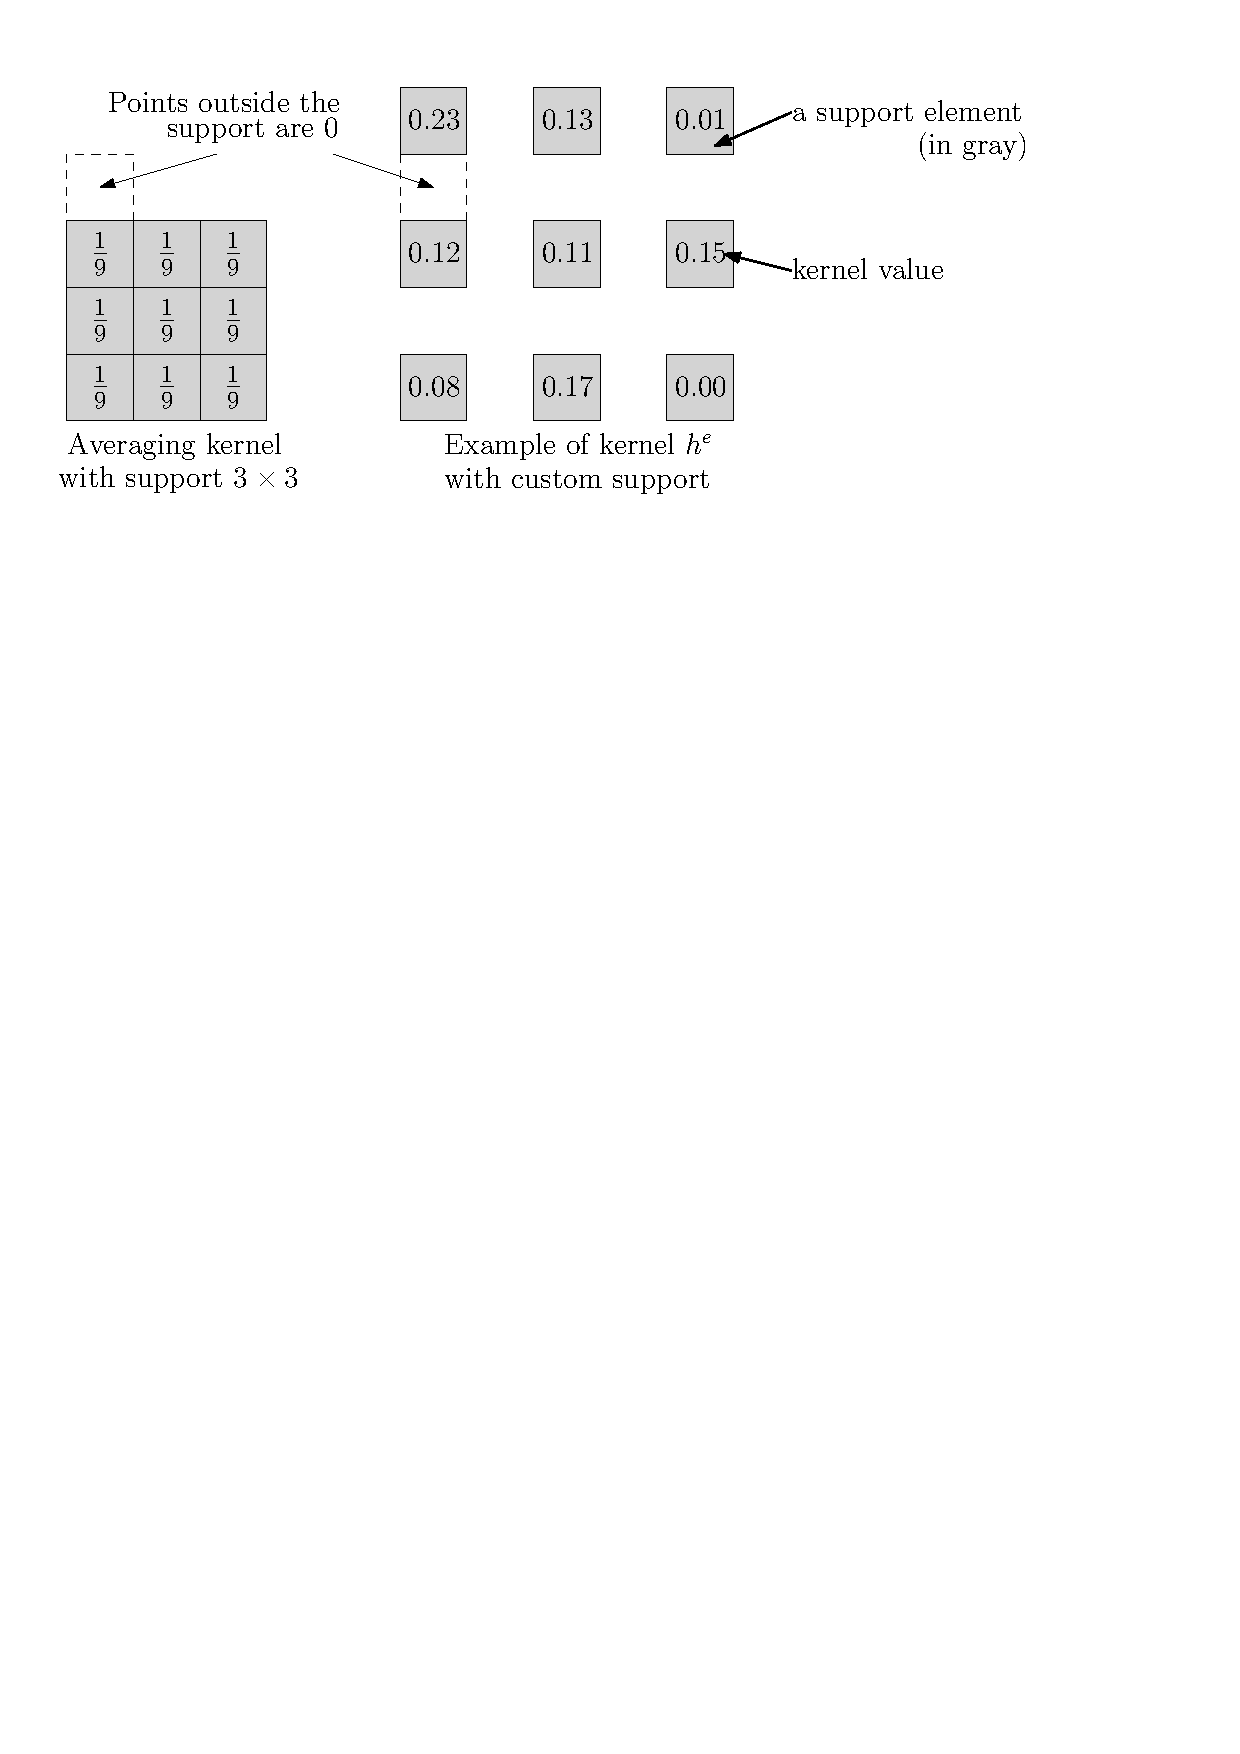
\includegraphics[width=0.8\textwidth]{figures/example-kernel.pdf}
\caption{(a) A well-known averaging kernel, which has fixed support ($3\times3$) and fixed values. (b) Example of a kernel $h^e$. The locations of the gray squares and the values (e.g. $.01$) actually change during PALMTREE. The shape of this $h^e$ (like a chessboard) has been shown experimentally to work well. \label{fig_example_kernel}}
\end{figure}

One columns of the dictionary $D$, usually named "atom", corresponds to one the convolution of successive kernels on a given branch identified by the leaf $l$. We will denote that successive convolution by
\begin{flalign*}
&& H^{l} = & h^r * \dots * h^l  && \text{$\triangleright$ column/atom $l$ of $D$} \\
&&            = & h^{*l}
\end{flalign*}

Figure \ref{fig_matrix_vs_tree} outlines the relation between the tree, the atoms $H^l$ and the matrix form. The dictionary can be written using this notation
$$D = \begin{bmatrix}H^{l_1} & H^{l_2} & \dots & H^{l_L}\end{bmatrix}$$
with $L$ the number of leaves in the tree. 

\begin{figure}[!h] \centering
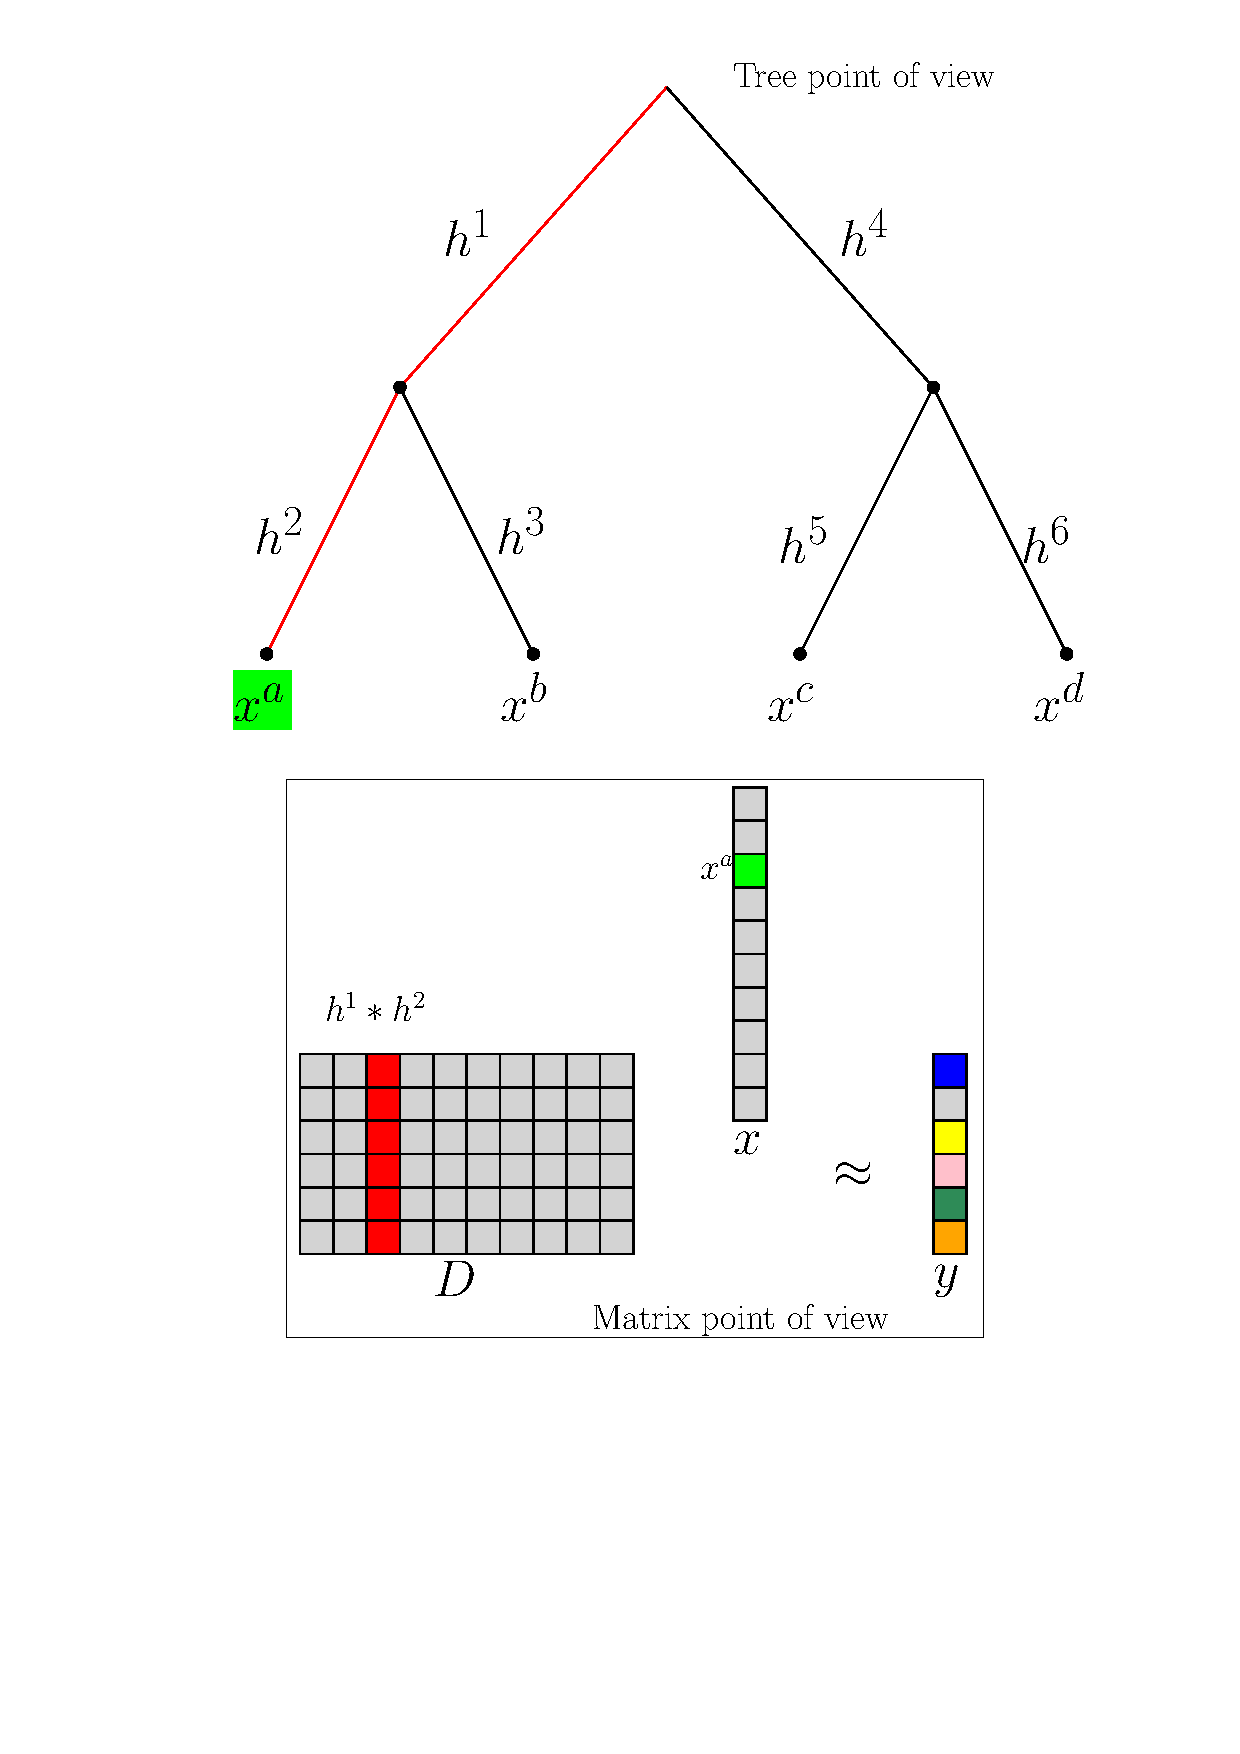
\includegraphics[width=0.9\textwidth]{figures/matrix-vs-tree.pdf} \caption{This figure shows how to go from the tree defined by its kernels $(h^e)_e$ to a matrix $D$. Note that this figure doesn't illustrates $Dx \approx y$ (standard matrix-vector product). Instead, it uses $D*x\approx y$ (convolutional product) which gives every possible translation for every atom.  \label{fig_matrix_vs_tree}}
\end{figure}
Now that $D$ is correctly defined, let's talk about $x$, the sparse representation that approximates $y$. As seen above, we use a convolution instead of the standard matrix-vector product:

$$D(x) = D*x \approx y$$
Note that $x$ belongs to $\mathbb{R}^{L\times N}$, $D$ has dimensions $N \times L$ and $y$ belongs to $\mathbb{R}^N$. To sum up the whole $D(x)$ operation:

$$
D(x) = \sum_{l \in \leaves} x^{l} * h^{*l}
$$
where $h^{*l}$ denotes the successive convolution of every kernel on the branch that leads to leaf $l$. Figure \ref{fig_matrix_vs_tree} shows an example with the branch $l=4$.

\section{The (FTL) problem}

The dictionary update step is defined as 
\begin{align}
(FTL) \quad \underset{\substack{(h^\text{e})_{e}}}\min & \lVert D(x) - y \rVert_2^2 \label{eq_ftl_energy}\\
\text{s.t. } & h^e_p = 0 \Rightarrow  s^e_p=0 \quad & \forall e \in 1..E, \forall p \in 1..N \label{eq_ftl_in_support} \\
 & \lVert h^e \rVert \le \gamma \label{eq_ftl_kernel_finite_nrj}
\end{align}

In the following, we will use the notation $(h^e)_{e}$ to denote $(h^e)_{e \in \mathcal{E}}$ . Also, the notation $\Phi((h^e)_{e})$ will denote the objective function (or energy) \ref{eq_ftl_energy}.
The constraint \ref{eq_ftl_in_support} guarantees that each kernel $h^e$ only has non-zero values on its support $s^e$. \ref{eq_ftl_kernel_finite_nrj} constrains the overall energy of every support to be finite and prevents a specific kernel to "explode".

\begin{figure}[!ht] \centering
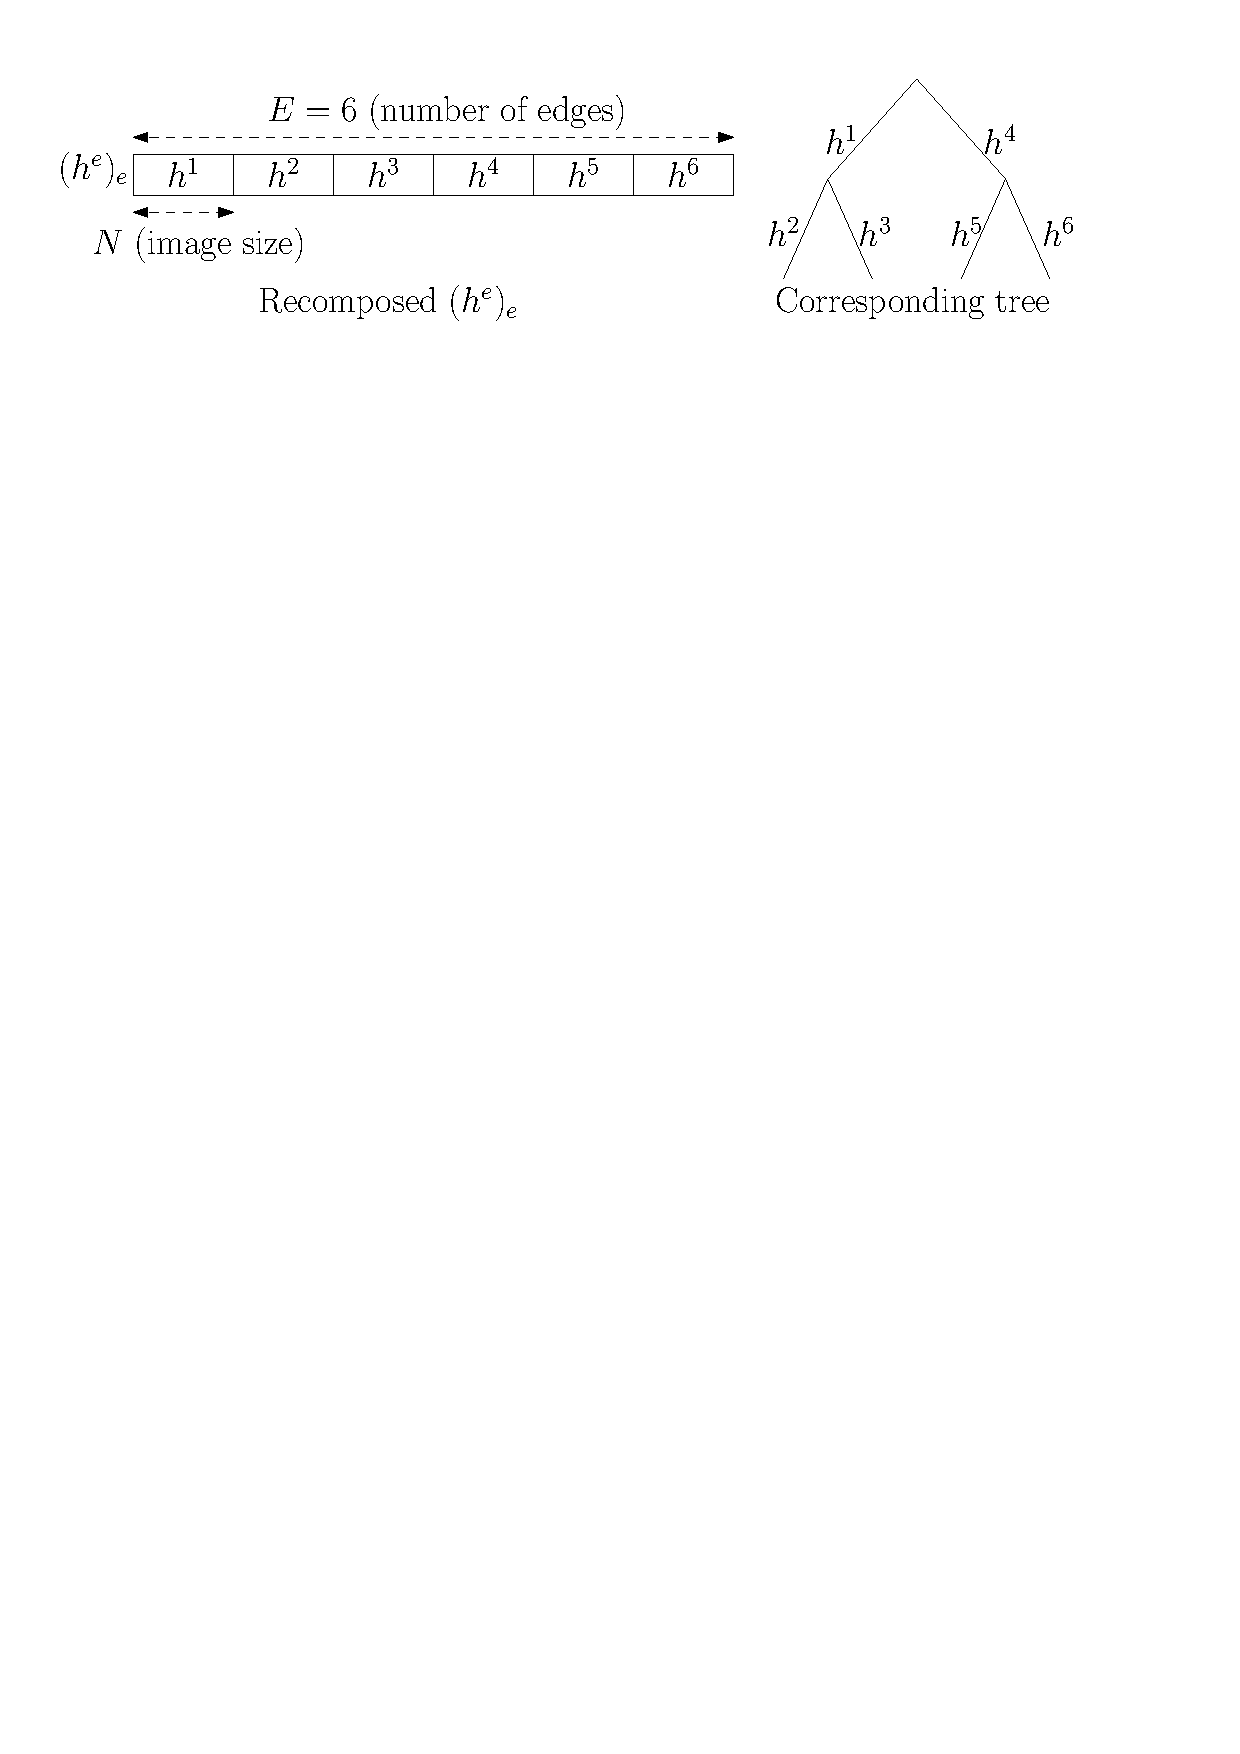
\includegraphics[width=0.8\textwidth]{figures/hk_tree.pdf}
\caption{A view of $(h^e)_e$ that "condenses" the dictionary information. In the (FTL) problem, $(h^e)_e$ is the variable to be minimized. $x^l$is fixed at all time.}\label{fig_hk_tree}
\end{figure}

(FTL) can be rewritten as an unconstrained problem, shifting the constraint spaces $(X^e)_e$ to the objective function using the characteristic function $\chi_{X^e}$defined for one edge $e$:
$$\chi_{X_e}(h^e) = \begin{cases} 0 &\text{ if } h^e \in X^e \\ +\infty & \ \text{otherwise}\end{cases}$$
(FTL) becomes

\begin{align}
(FTL) \quad \underset{\substack{(h^\text{e})_{e}}}\min & \lVert D(x) - y \rVert_2^2 + \sum_{e}\chi_{X_e} (h^e)
\end{align}

\subsection{Interesting (FTL) properties}
We may consider $D(x)$ as a polynomial form (see \ref{proof_ftl_polynomial}) ...

\subsection{PALMTREE, the algorithm for solving (FTL)}
...

\section{Issues with PALMTREE algorithm and internship goals}
As explained in \cite[p. 23]{chabiron_optimization_2016}, the main drawbacks to use this convolutional tree model for practical dictionary learning (as many other applications) are the hand-made parts of the model, leading to arbitrary and sub-optimal results. Among them are the design of the tree (degree, depth...) and the choice of the supports.
\subsection{Choice of the tree}
The paper chooses to use a fixed tree structure, meaning that the tree (degree, depth) has been created \emph{ad-hoc} on a per-experiment basis, trying to mimic the frequency pyramid tiling of a curvelet decomposition. The number of leaves was also specifically chosen to match the number of atoms that was generated on the target image.

But getting an actual adaptative dictionary update step implies that designing the tree is made optimally and as part of the optimization process. This is one of the internship research axis.

\subsection{Choice of the kernel supports}

As described in \ref{sec_tree_model}, the supports $s^e$ are part of the dictionary-as-a-tree model. In \cite{chabiron_toward_2015}, the authors experimentally show that using fixed supports for approximating curvelets is possible. For that specific purpose, the results turned to be good. But the whole model was supposed to be able to approximate any kind of image, hence the need for "adaptative" supports instead of hand-made ones. Figure \ref{fig_example_kernel} shows in dashed-line squares the hand-made support. The gray square show what we would expect from an "adaptive" support. Instead of keeping the same shape for every target atom, the supports evolves and get closer to the target shape.

And as for the tree design, the choice of where are located the elements of each kernel support has been made (so far) arbitrarily. The support of the $h^e$ kernel of fig. \ref{fig_example_kernel} shows an example of typical layout chosen for the experiments in \cite{chabiron_optimization_2016}. 

But our goal is to be able to approximate any kind of atoms, as \ac{KSVD} is able to do. Being able to choose what elements should be in the kernel supports as part of the optimization process is another goal during this internship.

\begin{figure}[!ht] \centering
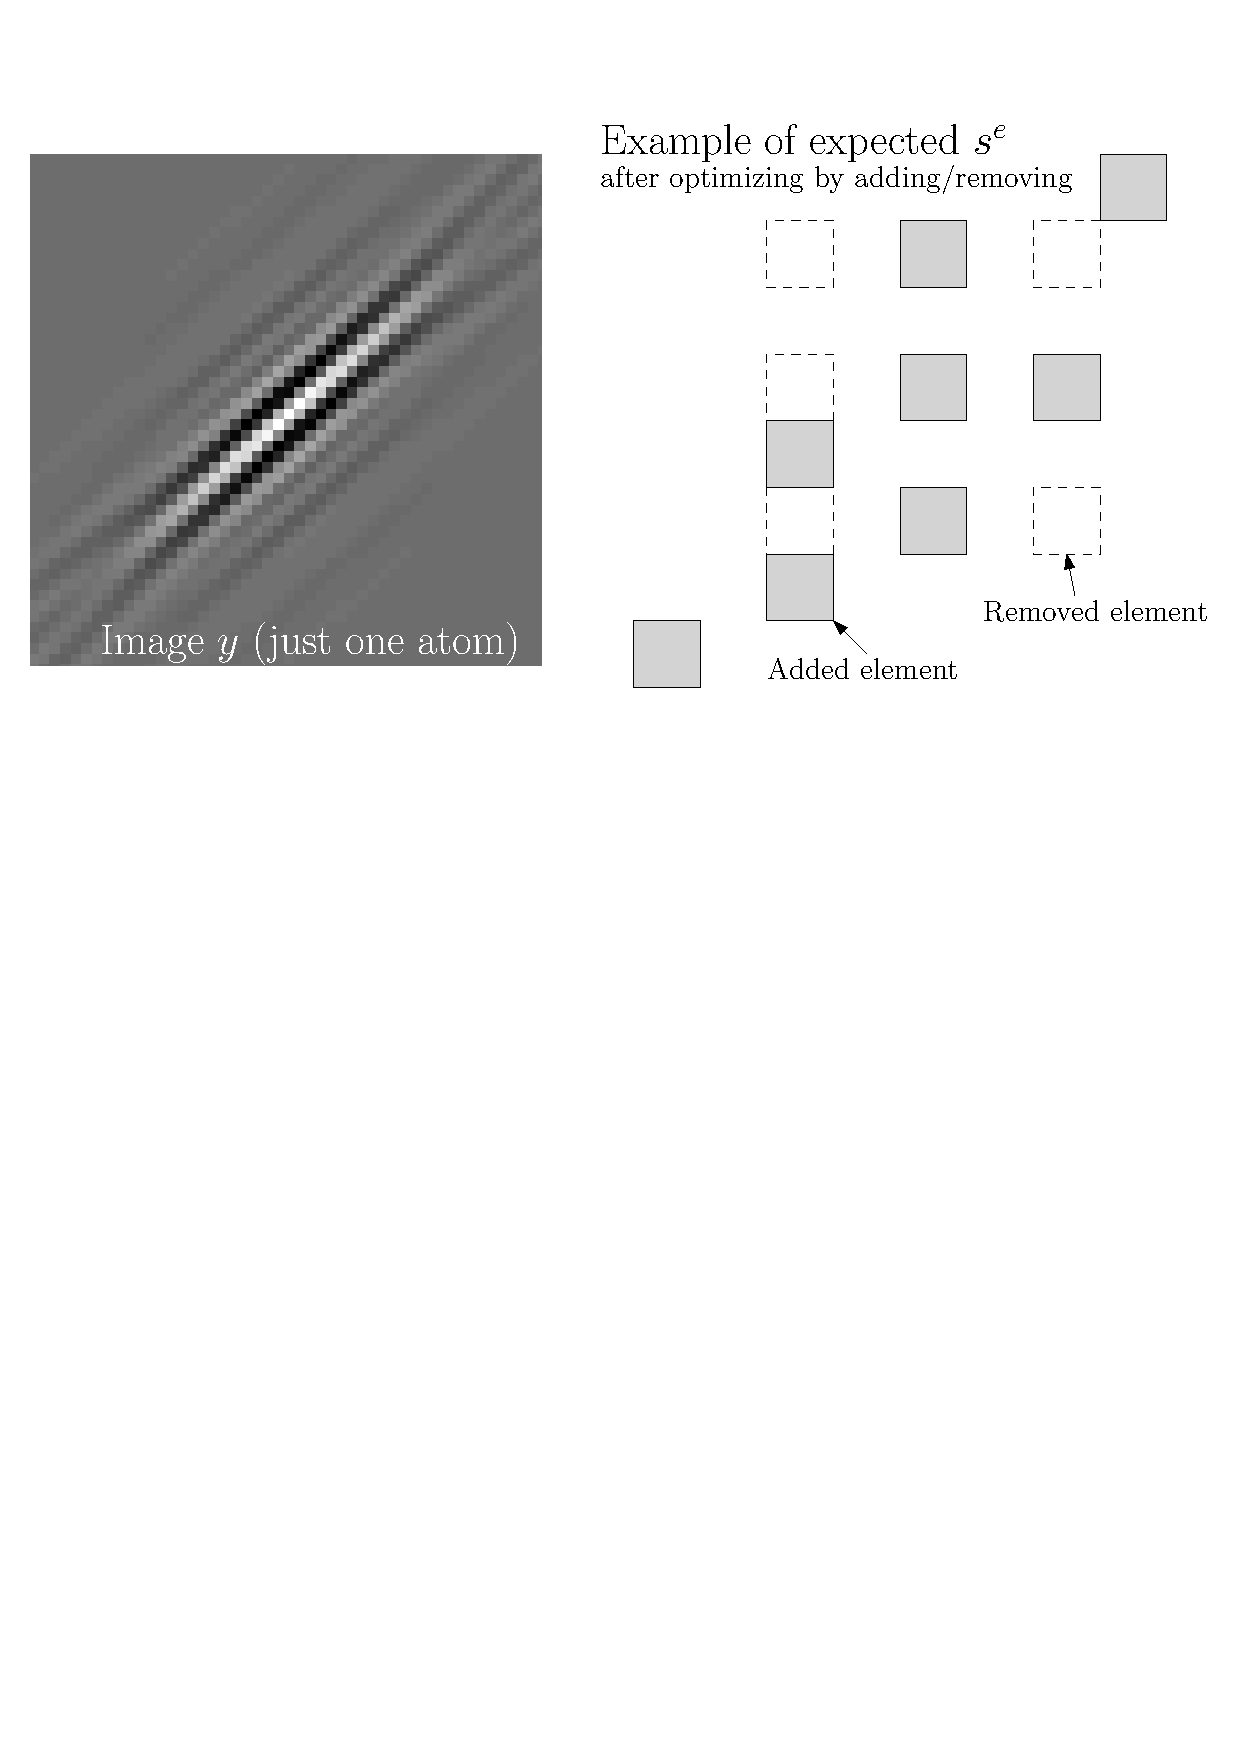
\includegraphics[width=0.6\textwidth]{figures/add-rm-elmts-support.pdf}
\caption{On the left, a simple curvelet atom which serves as target image. The right figure represents the locations of the support element for one of the kernels of the tree. The dashed squares represent the initial support given in figure \ref{fig_example_kernel}. The gray squares show the (supposedly) locations of the support elements after optimization. The elements have moved to the general direction of the curvelet.\label{fig_example_optimal_support}}
\end{figure}

\chapter{Experiments}

\section{First research axis: experimenting with adaptative supports}

After being able to correctly add and remove support elements, the second phase was to think about what elements we would add or remove, and when (i.e. when during the PALMTREE algorithm).

The figure \ref{fig_example_optimal_support} shows an example of what we think would happen when allowing to add and remove elements: the support would shape itself to better match the target atom (in fig.\ref{fig_example_optimal_support}, the atom shown is actually the whole target image).


\subsection{Adding an element}
Our first thought on how to add an element to a support was to find the best kernel among the tree edges, and then pick the best point(s) of that support to be added. We thought the gradient of the objective function would probably give that information. 

...explain...

\subsection{Experiment 1: knowing what elements are worth adding}

This experiment was using a single-branch tree of depth 4 (see fig. \ref{fig_xp_pts_worth_adding}). One of the four supports is picked for the whole experiment. This support will be called $s^e$.
\begin{figure}[!ht]\centering
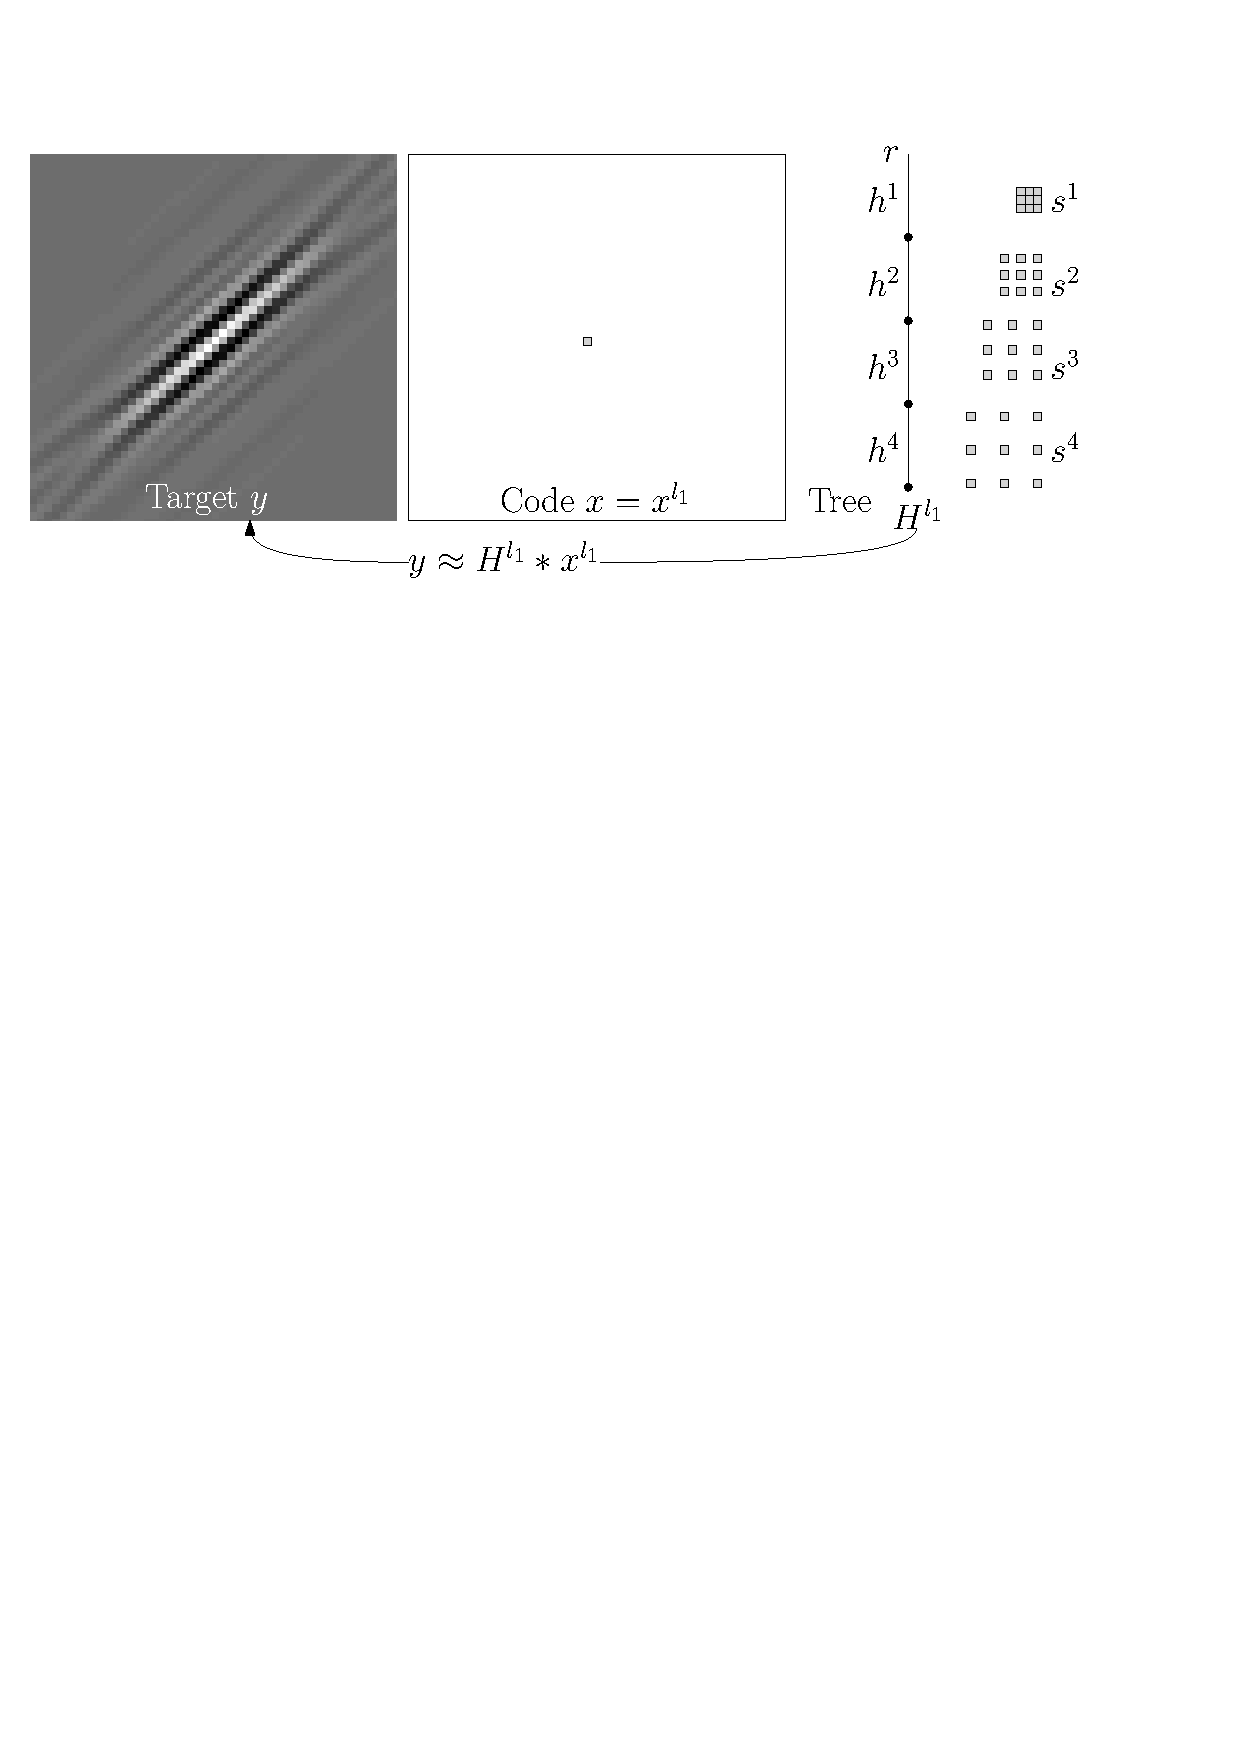
\includegraphics[width=0.8\textwidth]{figures/xp-pts-worth-adding.pdf}
\caption{a} \label{fig_xp_pts_worth_adding}
\end{figure}
First, a full minimization with many iterations and retries is made to give a common starting point. Then, for every (not already at 1) element $i \in \mathcal{P}$  of the support $s^e$, the element is added to the support, and the minimization continues (with no retries to get the same conditions for every added point).
The objective function of that minimization is then stored so that the location of $i$ is remembered. The element $i$ is then removed and we continue with $i+1$...

As a result, we get an image that represent, for each pixel, the minimized objective function if an element were added at that specific location. This extremely slow method allows us to compare with faster methods (like just computing the gradient).


\subsection{Experiment 2: use the gradient for choosing what should be added}
This experiment aims to simulate the choice of an atom by the OMP algorithm. As a short reminder, here is the step we are studying:
\begin{algorithm}[!ht] % XXX Finish algorithm
    \caption{MP (Matching Pursuit) algorithm for sparse approximation}
  \begin{algorithmic}[0]
    \Input signal $y \in \mathbb{R}^{n}$, dictionary $D \in \mathbb{R}^{n \times m}$ with $m>>n$, $x = 0_{\mathbb{R}^m}$
    \Output Code $x$ which is $k$-sparse
    \State \textbf{Initialization} $R^{(0)} = y$
    \While{$i \leq k$} \Comment note the fixed number of iterations
      \State $l =  \arg\max_{l = 1,\dots,l} |\left< d_l,R^{(i)} \right>|$ \label{alg_omp_pick_correlation}
        \Comment{find atom with max. correlation with $R$}
      \State $R^{(i+1)} = R^{(i)}-x_l d_l^{(i)}$
      \State $\hat{y} = \hat{y}+\langle R^{(i)}, d_{l}^{(i)} \rangle d_{l}^{(i)}$
      \State $i = i + 1$
    \EndWhile
  \end{algorithmic}
\end{algorithm}

At \cref{alg_omp_pick_correlation}, the algorithm chooses the column of the dictionary that matches the best the residual. This is where we thought this way of doing would serve our "add an element to one of the supports" algorithm.

% XXX define PALMTREE
Our goal is to, between two iterations of the PALMTREE algorithm, add a new element to one of the supports. That would lead to an optimization-driven construction of the kernels instead of designing them by hand.

But we have been questioning ourselves on the fairness of choosing an element to be added based the mere partial gradient. We remind that the \ref{alg_omp_pick_correlation} is actually computing a gradient:

\begin{align*}
l =& \argmax \left|\left< g_l,R^{(i)} \right>\right| \\
=& \argmax \left| D^TR^{(i)}\right| \\
=& \argmax \left| D^T(D\alpha - u)\right| \\
\end{align*}
So: does the partial gradient \ref{eq_partial_gradient} give 
\begin{align*}
\Phi((h^e)_e) = \left\| \sum_{l\in\leaves} x^l * h^{*l} \right\|^2
\end{align*}
\begin{align*} 
\nabla_{h^{e'}}\Phi((h^e)_e) = 2 \widetilde{H^{e'}} * (h^{e'}*H^{e'}-y^{e'})
\end{align*} \label{eq_partial_gradient}


\section{Does the gradient give enough information to choose an element to be added to the support?}

After being able to add
\subsection{Results}
\begin{figure}[!h]\centering
    \begin{subfigure}[b]{0.49\textwidth}\centering
    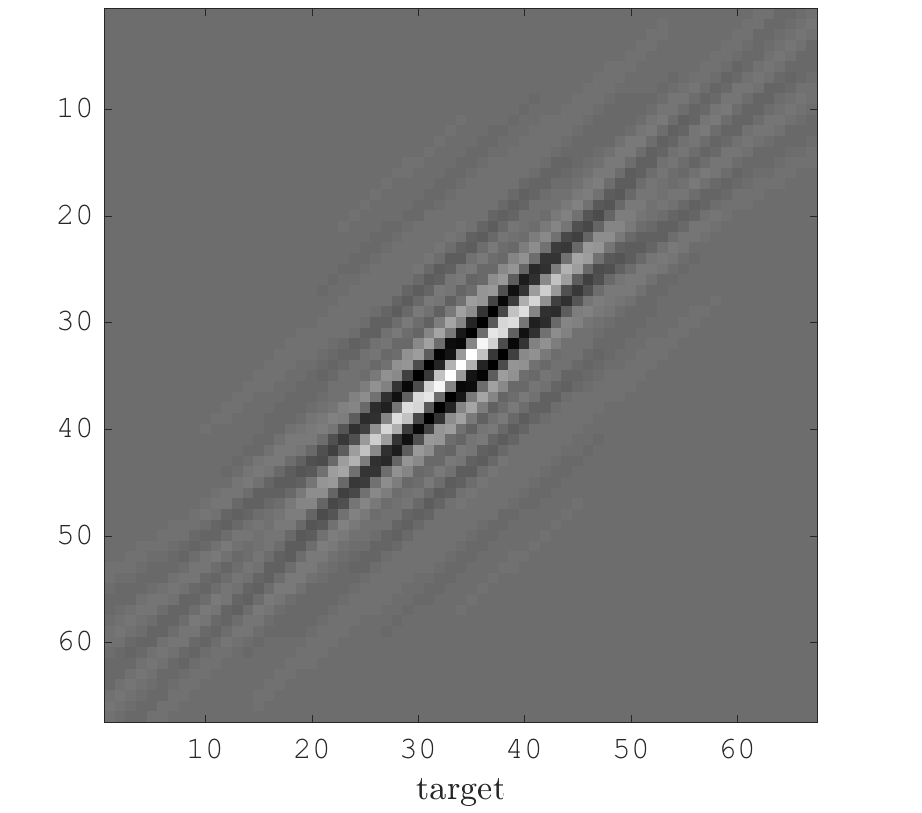
\includegraphics[width=\textwidth]{figures/xp/xp_128x128_sc2_angl1_K3_S3_node2_target.png}
    \end{subfigure}
\begin{subfigure}[b]{0.49\textwidth}\centering
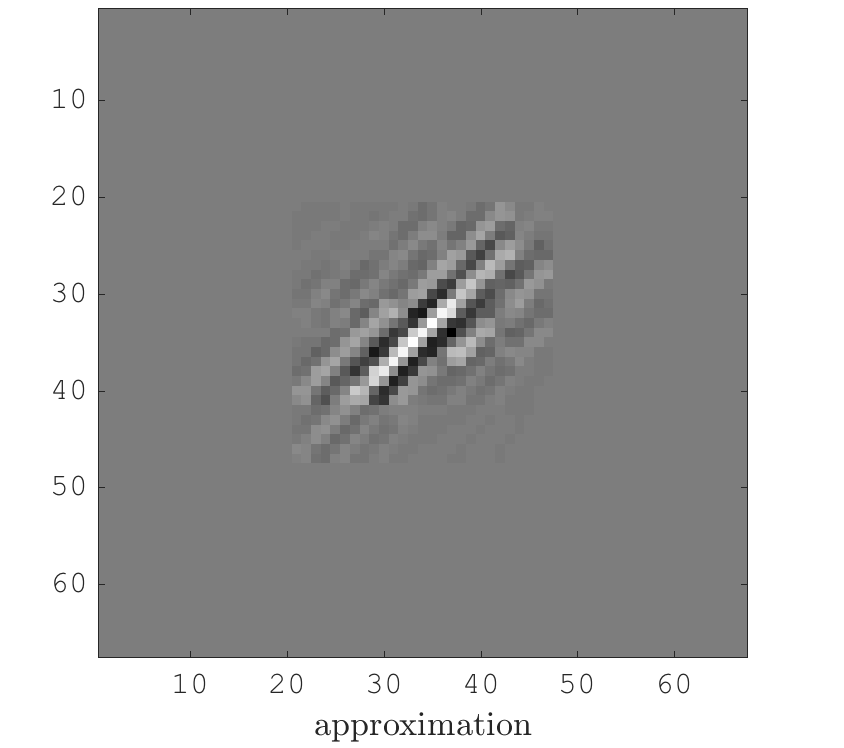
\includegraphics[width=\textwidth]{figures/xp/xp_128x128_sc2_angl1_K3_S3_node2_approx.png}
\end{subfigure}
   \begin{subfigure}[b]{0.49\textwidth}\centering
    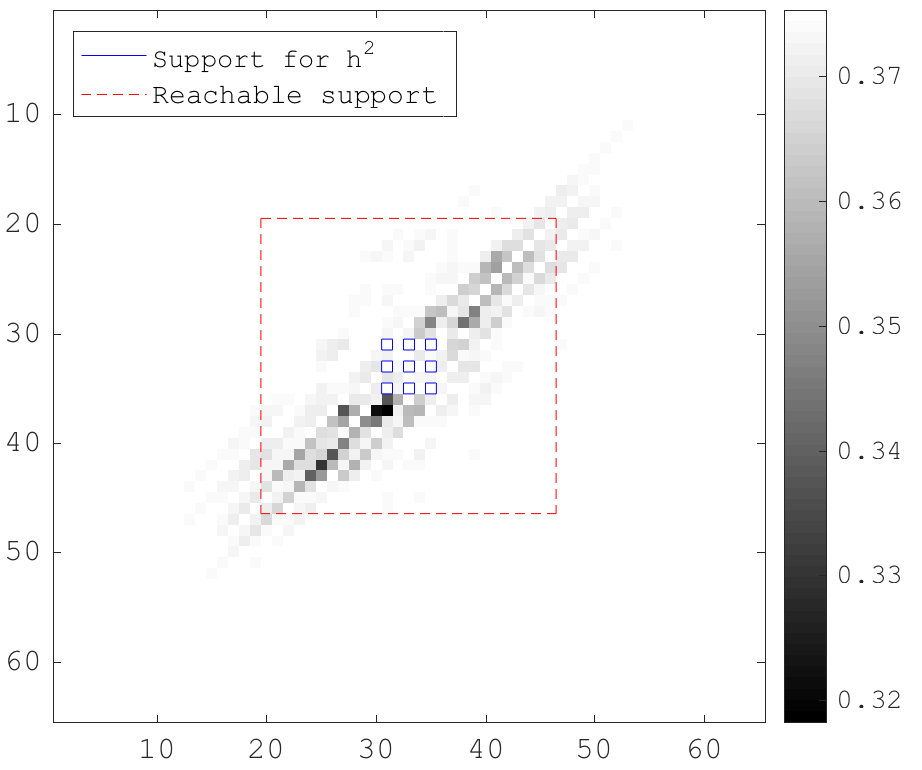
\includegraphics[width=\textwidth]{figures/xp/xp_128x128_sc2_angl1_K3_S3_node2_obj_matrix.png}
    \end{subfigure}
    \begin{subfigure}[b]{0.49\textwidth}\centering
    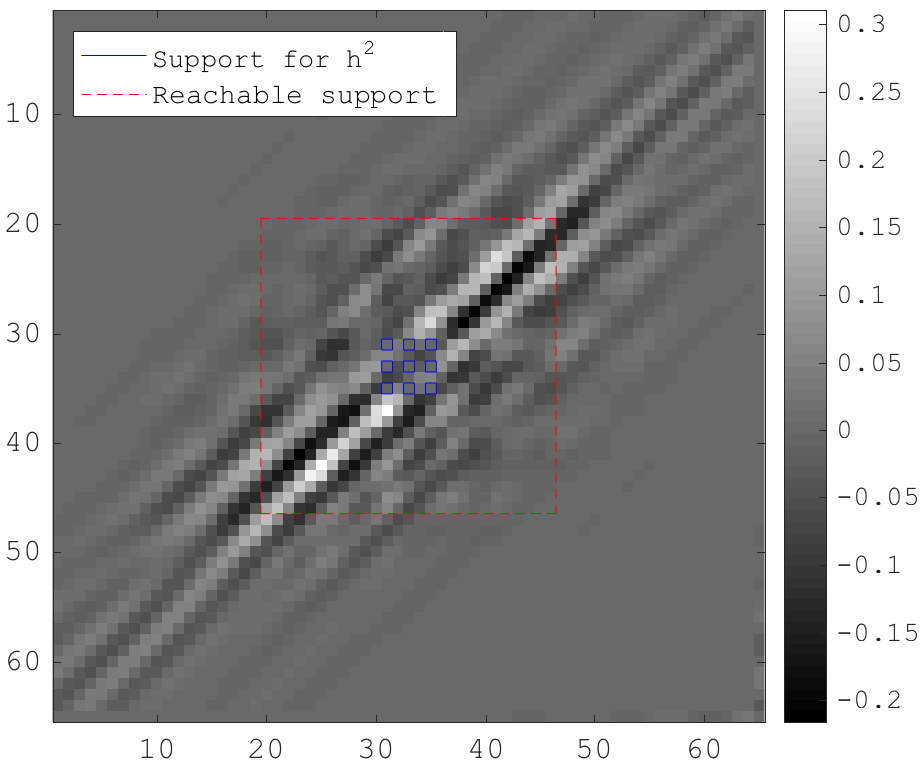
\includegraphics[width=\textwidth]{figures/xp/xp_128x128_sc2_angl1_K3_S3_node2_gradient_node_2.png}
    \end{subfigure}
\end{figure}

\begin{table}[!h]\centering
\begin{tabular}{@{}lll@{}}\toprule
 & RMSE & Relative RMSE \\ \midrule
Before & 0.004786 & 0\% \\
After & 0.004407 & 7.9\% \\ \bottomrule
\end{tabular}
\caption{RMSE comparison when adding to the support on the \nth{2} edge. Note that for the "added point" RMSE, we took the minimum of all RMSE for every point possibly added. Here, the RMSE is at best increased by 7.9\%.}
\end{table}


% XXX Proof not finished; this proof might be useless/overkill in my thesis...

\clearpage
\addcontentsline{toc}{chapter}{Appendix}
\appendix

\chapter{Some stuff I'm writing to remember things}

\section{Why is sparse coding used for denoising?}

The figure \ref{sparse_reduce_noise} shows a noisy signal $y$ living in a high-dimensional $N$ and defined by
$$y=\hat{y} + b$$
with $b$ following a centered Gaussian distribution $\mathcal{N}(0,\sigma^2I)$ and $\hat{y}$ the noise-less signal. We see that the distance $||b||$ is always lower than the projected distance.

This is because the deviation in the $N$ dimensional space can be written as
\begin{align*}
\sigma^2(b) =& \mathbb{E}\left[\lVert b-\mathbb{E}(b) \rVert^2 \right]\\
=& \mathbb{E}\left(\lVert b \rVert^2 \right)\\
=& ... \\
=& \frac{1}{N}\lVert b \rVert^2
\end{align*}
which gives 
$$ \lVert b \rVert = \sigma\sqrt{N} $$
When projected to the $K$ dimensional space, the noise deviation becomes
$$\lVert b \rVert = \sigma\sqrt{K} $$
which is much better than the previous distance, provided that $K<<N$. 

\begin{figure}[!h]\centering
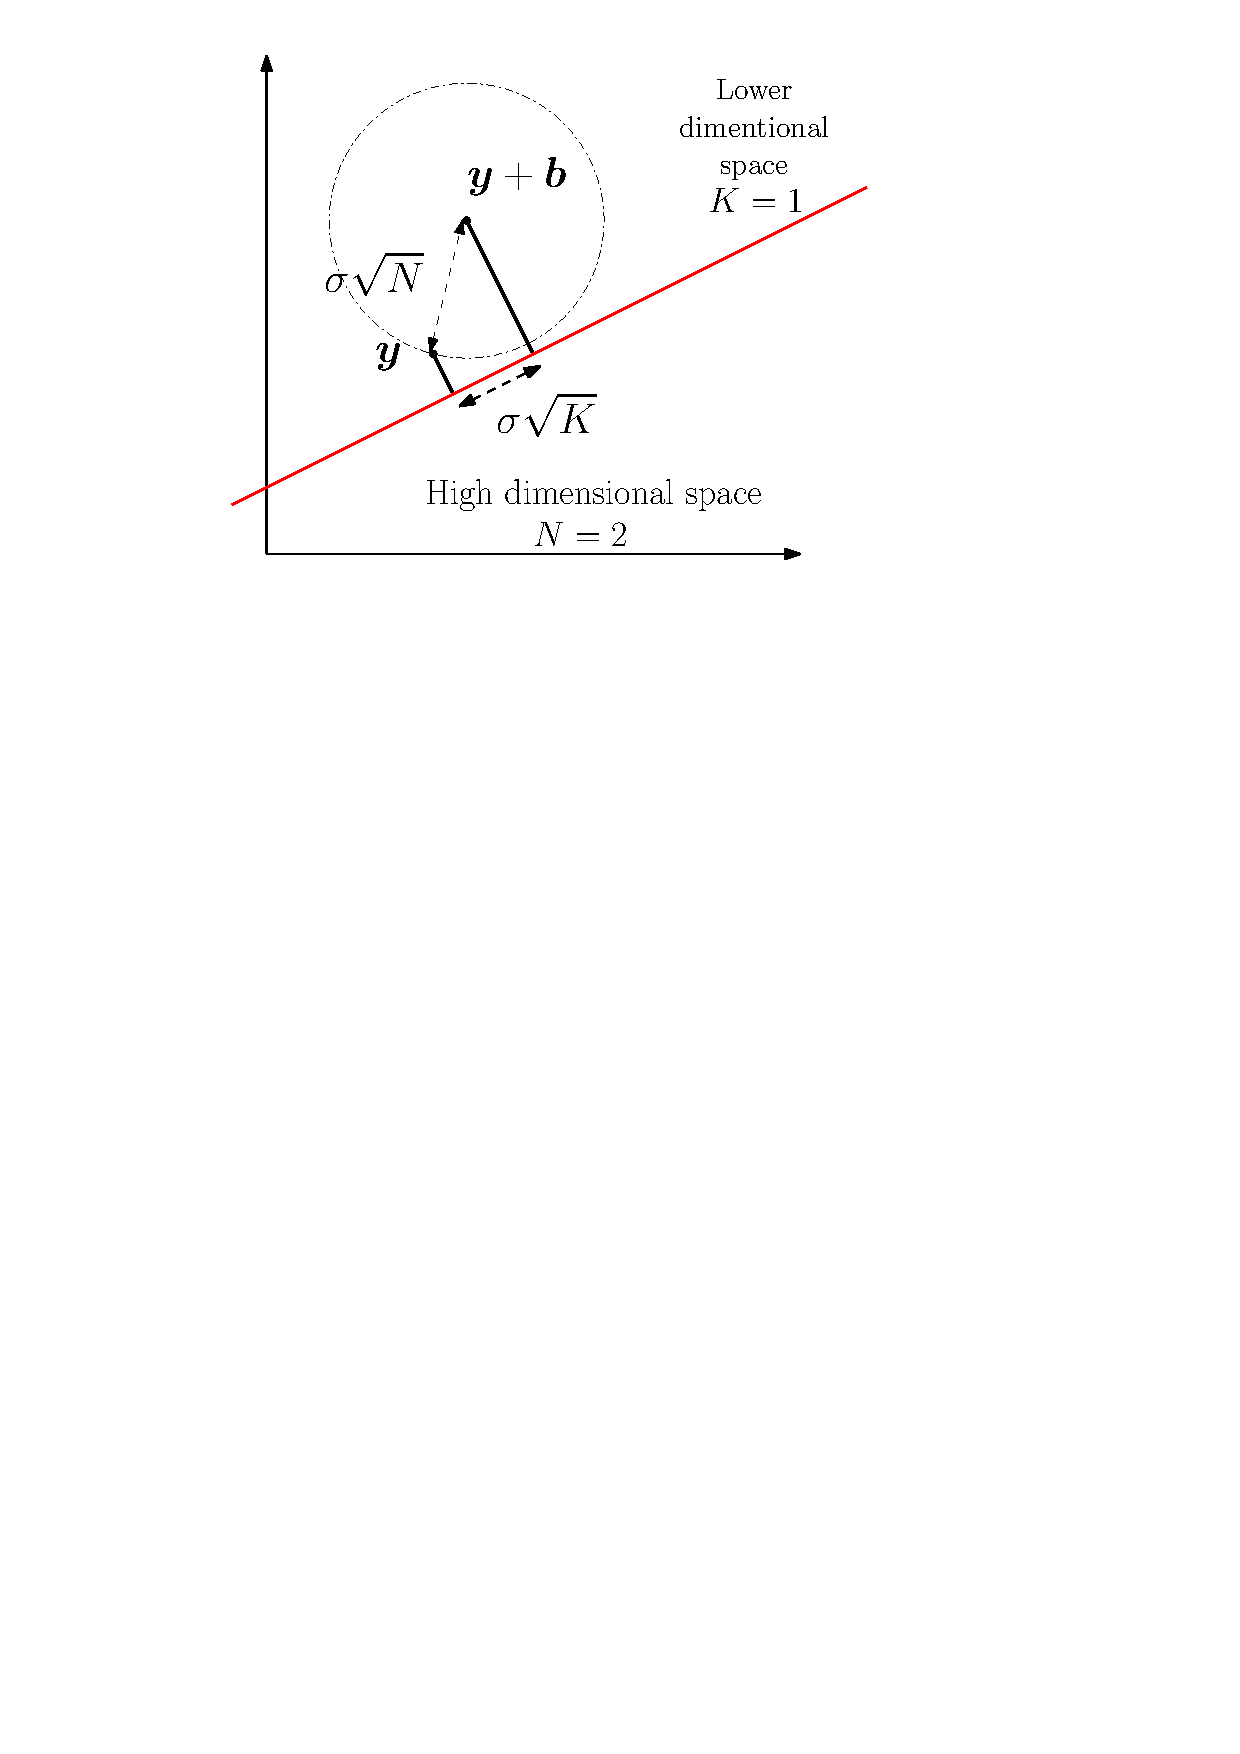
\includegraphics[width=0.5\textwidth]{figures/sparse-reduce-noise.pdf}
\caption{When projected onto a lower dimensional space, the standard derivation of the additive Gaussian noise $b \sim \mathcal{N}(0,\sigma^2)$ will be greatly reduced if $K<<N$. The sparser the representation the better the denoising. \label{sparse_reduce_noise}}
\end{figure}

\section{Why $FT(\widetilde{A}) = FT(A)^*$}
\begin{align*}
(\widehat{\widetilde{A}})_{m,n} =& \sum_{k=1}^M \sum_{l=1}^N \widehat{A}_{k,l} e^{-2i\pi (k\frac{m}{M}+l \frac{n}{N})}\\
=& \sum_{k=1}^M \sum_{l=1}^N A_{-k,-l} e^{-2i\pi (k\frac{m}{M}+l \frac{n}{N})}\\
\shortintertext{By changing variables $k'=-k$ and $l'=-l$, we get:}
=& \sum_{k'=-M}^{-1} \sum_{l'=-N}^{-1} A_{k',l'} e^{2i\pi (k'\frac{m}{M}+l' \frac{n}{N})}
\shortintertext{And thanks to the $(M,N)$ periodicity of $A$, which means that $A_{i,j}=A_{i+kM,j+lN}$, $\forall (k,l) \in \mathbb{N}^2$, letting us with:}
=& \sum_{k'=-M}^{-1} \sum_{l'=-N}^{-1} A_{k'+M,l'+N} e^{2i\pi (k'\frac{m}{M}+l' \frac{n}{N})}\\
\shortintertext{With a second change of variables $k''=k'+M$ and $l''=l'+N$:}
=& \sum_{k''=-M+M}^{-1+M} \sum_{l''=-N+N}^{-1+N} A_{k'',l''} e^{2i\pi (k'\frac{m}{M}+l' \frac{n}{N})}\\
=& \sum_{k'=1}^{M} \sum_{l'=1}^{N} A_{k',l'} e^{2i\pi (k'\frac{m}{M}+l' \frac{n}{N})}
\end{align*}


\printbibliography

\end{document}



